\documentclass{article}
\usepackage[a4paper,margin=28mm]{geometry}
\usepackage{lmodern}
\usepackage[numbers,sort&compress]{natbib}
% BEGIN inlined from preamble

\usepackage[utf8]{inputenc}
\usepackage[T1]{fontenc}
\usepackage{amsmath,amssymb,amsthm}
\usepackage{graphicx}
\usepackage{subcaption}
\usepackage{tikz}
\usetikzlibrary{arrows.meta,calc,backgrounds,positioning}
\usepackage{mathtools}
\usepackage{xr-hyper}
\usepackage{hyperref}
\hypersetup{hidelinks}
\usepackage{url}
\usepackage{booktabs}
\usepackage{nicefrac}
\usepackage{microtype}
\usepackage{xcolor}
\definecolor{helperorange}{RGB}{255,229,204}
\definecolor{helperdarkorange}{RGB}{190,95,0}

\usepackage{enumitem}
\usepackage{longtable}
\usepackage{bm}
\usepackage{dsfont}
\newcommand{\argmin}{\mathop{\mathrm{arg\,min}}}
\newcommand{\argmax}{\mathop{\mathrm{arg\,max}}}
\newcommand{\dotp}[2]{\langle #1,#2 \rangle}
\theoremstyle{plain}
\newtheorem{theorem}{Theorem}[section]
\newtheorem{lemma}{Lemma}[section]
\newtheorem{proposition}{Proposition}[section]
\newtheorem{corollary}{Corollary}[section]
\newtheorem{definition}{Definition}[section]
\newtheorem{remark}{Remark}[section]
\newcommand{\mc}[1]{\mathcal{#1}}
\newcommand{\tn}[1]{\textnormal{#1}}
\newcommand{\ones}{\mathds{1}}
\newcommand{\entropy}{H}
\newcommand{\Vertex}{V}
\newcommand{\Edge}{E}
\newcommand{\EdgeIndicator}{1_{\Edge}}
\newcommand{\length}{W}
\newcommand{\lengthSet}{\mc{W}}
\newcommand{\prob}{\tn{Prob}}
\newcommand{\WD}{{\tn{W}}}
\newcommand{\flows}{\mc{F}}
\newcommand{\flowsCol}{C}
\newcommand{\softmin}{\tn{smin}}
\newcommand{\hinge}{h}
\newcommand{\veps}{\varepsilon}
\newcommand{\transp}[1]{ {#1}^{\top} }
\newcommand{\enscond}[2]{ \left\{ #1 \;:\; #2 \right\} }
\newcommand{\eqdef}{\coloneqq}
\newcommand{\eq}[1]{\begin{equation*}#1\end{equation*}}
\newcommand{\eql}[1]{\begin{equation}#1\end{equation}}
\DeclareMathOperator{\diverg}{div}
\newcommand{\RR}{\mathbb{R}}
\newcommand{\ZZ}{\mathbb{Z}}
\newcommand{\Ll}{\mathcal{L}}
\newcommand{\RRPInf}{{\overline{\RR}}}
\newcommand{\Cc}{\mathcal{C}}
\newcommand{\pa}[1]{\left( #1 \right)}
\DeclareMathOperator{\Proj}{Proj}
\newcommand{\qandq}{ \quad \text{and} \quad }
\DeclareMathOperator{\diag}{diag}
\newcommand{\al}{\alpha}
\newcommand{\be}{\beta}
\renewcommand{\epsilon}{\varepsilon}
\DeclareMathOperator{\sign}{sign}
\renewcommand{\it}[1]{#1^{(k)}}
\newcommand{\itt}[1]{#1^{(k+1)}}
\newcommand{\range}{\operatorname{range}}
\newcommand{\norm}[1]{\|#1\|}
\newcommand{\Umax}{U_\gamma}
\newcommand{\Xmax}{X_\gamma}
\newcommand{\XmaxZero}{X_0^\star}
\newcommand{\XmaxGamma}{X_\gamma^\star}
\newcommand{\Vnorm}[1]{\norm{#1}_V}
\newcommand{\norminf}[1]{\norm{#1}_\infty}
\DeclareMathOperator{\arsinh}{arsinh}
\newcommand{\normVar}[1]{\norm{#1}_{\mathrm{Var}}}
\newcommand{\z}{z}
\newcommand{\zC}{\z^C}
\newcommand{\KL}{\mathrm{KL}}
\newcommand{\KLdiv}[2]{\mathrm{KL}(#1|#2)}
\newcommand{\Xx}{\mathcal{X}}
% END inlined from preamble

\DeclareMathOperator{\tr}{tr}
\newcommand{\opnorm}[1]{\lVert #1\rVert_{\mathrm{op}}}
\newcommand{\nucnorm}[1]{\lVert #1\rVert_*}
\newcommand{\Dhop}{D_{\mathrm{hop}}}
\newcommand{\Dweight}{D_W}
\setlength{\emergencystretch}{2em}
\title{Robust Sublinear Convergence Rates\\for Iterative Bregman Projections}
\author{Gabriel Peyr\'e\\CNRS and \`Ecole normale sup\'erieure, PSL University\\
\texttt{gabriel.peyre@ens.fr}}
\date{}
\begin{document}
\maketitle
\begin{abstract}
Entropic regularization provides a simple way to approximate linear programs whose constraints split into tractable blocks. The resulting objectives admit alternating Kullback--Leibler (KL) projections, including Sinkhorn scaling for optimal transport. We give a convergence blueprint separating three ingredients: bounded primal masses, bounded dual potentials in a quotient seminorm, and a residual-to-gap estimate. The dual gap is at most $8X_\gamma U_\gamma^2\lVert A\rVert_{1\to1}^2/(\gamma k)$; the dependence of the bounds $X_\gamma,U_\gamma$ on the regularization $\gamma$ is part of the guarantee, not suppressed in it. We establish the required bounded-mass Pinsker inequality without assuming that successive projections have equal mass. For graph Wasserstein--1 transport, a lifted splitting yields sparse flow-Sinkhorn updates costing $O(p)$ per sweep, where $p$ counts directed edges. Explicit constants imply an $O(p\varepsilon^{-3})$ arithmetic bound for estimating the unregularized optimal value on a fixed graph, rather than a guarantee on a feasible flow at each iterate. Experiments illustrate the regularization--runtime tradeoff on synthetic and single-cell graphs. We also discuss balanced transport, general Bregman divergences, quantum transport, and the precise scope of an accompanying, partially formalized Lean development.
\end{abstract}
\section{Introduction}
Iterative Bregman projections turn structured constrained optimization into alternating normalization steps. Their sparse linear algebra and GPU-compatible updates are useful in machine learning, notably for optimal transport, barycenters, and unbalanced transport~\citep{Cuturi13,benamou2015iterative,chizat2018scaling}. A general convergence blueprint helps identify which properties make these methods effective and which constants deteriorate when the regularization is reduced.

\paragraph{Bregman projections and iterative scaling.}
Alternating projections originate in Bregman's method~\citep{Bregman67} and the information-geometric analysis of Csisz\'ar and Tusn\'ady~\citep{CsiszarTusnady84}; a general convex-analytic treatment is given in~\citep{BauschkeBorwein1997}. Iterative proportional fitting and matrix scaling have a long history~\citep{DemingStephanIPFP,Sinkhorn64}. For positive transport kernels, projective-metric contraction gives linear convergence~\citep{FranklinLorenz89,borwein1994dad}, but the resulting contraction factor can approach one exponentially fast as $\gamma$ decreases. We instead study a weaker quantity, the dual objective gap, with explicit polynomial dependence on the regularization. This does not imply equally sharp primal-distance convergence.

\paragraph{Robust transport bounds.}
Polynomial complexity estimates for scaling and entropic transport were developed in~\citep{kalantari2008complexity,altschuler2017near,dvurechensky2018computational,chakrabarty2021sinkhornsublinearrate}; related perspectives use mirror descent~\citep{leger2021gradient,aubin2022mirror}. For balanced probability marginals, bounded mass leads to an $O(1/(\gamma k))$ dual rate. More generally, a rate written as $O(X_\gamma U_\gamma^2/(\gamma k))$ is only as robust as the bounds on $X_\gamma$ and $U_\gamma$. In particular, our graph-flow bound has $X_\gamma=O(1/\gamma)$, giving $O(1/(\gamma^2k))$ for fixed graph data. Linear-rate refinements under additional assumptions are complementary~\citep{chizat2025sharper}; neither kind of estimate eliminates the statistical and computational tradeoffs of choosing $\gamma$.

\paragraph{Transport on graphs.}
For a shortest-path ground metric, Wasserstein--1 transport admits a minimum-cost flow formulation, the discrete counterpart of Beckmann's formulation~\citep{Beckmann52,AhujaEtAl93}. Tree distances even admit closed-form transport costs~\citep{evans2012phylogenetic}. General networks admit sophisticated exact and approximate flow algorithms~\citep{orlin1993minimum,daitch2008faster}; our contribution is not a better worst-case dependence on accuracy than these solvers. It is a simple sparse entropy-regularized iteration with an explicit convergence analysis. Applying vanilla Sinkhorn to graph transport instead acts on the generally dense shortest-path distance matrix: setting non-edge costs to $+\infty$ would forbid direct coupling of nonadjacent vertices, not allow routing through them, and defines a different transport problem. Dense rounding results~\citep{altschuler2017near} remain applicable to the dense formulation, without removing this quadratic storage and update bottleneck.

\paragraph{Contributions.}
The core contribution is a general blueprint for iterative KL projections and its instantiation in a sparse flow-Sinkhorn algorithm. Figure~\ref{fig:blueprint} links the two main results, Theorems~\ref{thm:kl-dual-rate} and~\ref{thm:approx-linprog}, to the primal and dual helpers, Propositions~\ref{prop:mass-bound-block} and~\ref{prop:uniform-iter-final}. The graph application gives $O(p)$ sweeps and a fully specified optimal-value guarantee (Theorem~\ref{thm:graphw1-complexity}); CPU and GPU experiments on synthetic and genomic-inspired graphs illustrate the tradeoff between regularization bias and runtime. Balanced transport provides a second complete instantiation (Appendix~\ref{app-app:sinkhorn-ot}). Quantum transport is a promising further example, particularly for quantum-information and quantum-machine-learning problems: its trace-norm Pinsker geometry fits the Bregman blueprint, but our explicit quotient-norm/non-expansiveness route is not yet established for its dual block maps. Existing quantum Sinkhorn convergence and dual estimates must be distinguished from this remaining step (Appendix~\ref{app-app:quantum-ot}). Code, benchmarks, and the Lean development are available at \url{https://github.com/gpeyre/flow-sinkhorn}; Appendix~\ref{app-sec:lean-formalization} states the formalization's current limitations. Auxiliary non-expansiveness and general Bregman arguments are in Appendices~\ref{app-sec:non-expansiveness} and~\ref{app-app:general-bregman}.

\begin{figure}[htbp]
\centering
\resizebox{\linewidth}{!}{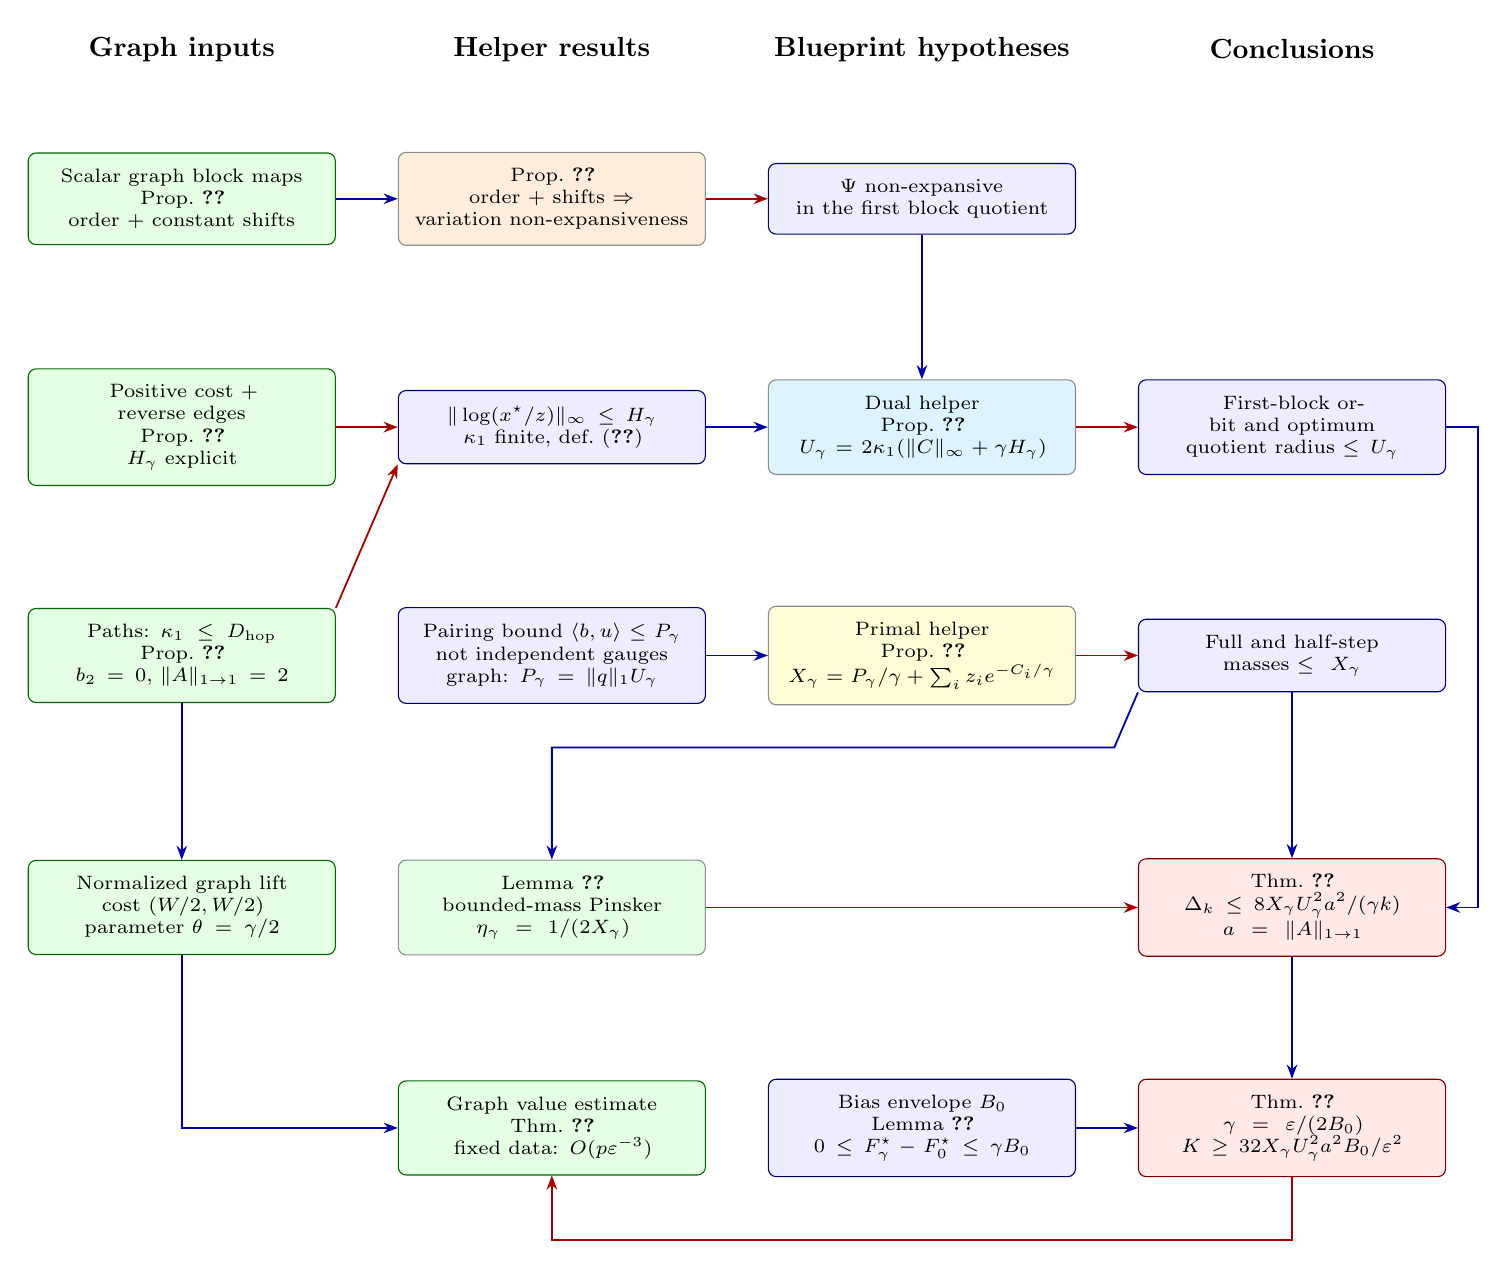
\begin{tikzpicture}[x=1mm,y=-1mm,font=\scriptsize,
 hypothesis/.style={draw=blue!45!black,fill=blue!7,rounded corners=1mm,align=center,inner sep=2mm,text width=35mm},
 result/.style={draw=red!50!black,fill=red!9,rounded corners=1mm,align=center,inner sep=2mm,text width=35mm},
 helper/.style={draw=black!45,fill=yellow!16,rounded corners=1mm,align=center,inner sep=2mm,text width=35mm},
 graph/.style={draw=green!40!black,fill=green!10,rounded corners=1mm,align=center,inner sep=2mm,text width=35mm},
 barr/.style={-{Stealth[length=1.8mm]},blue!65!black,line width=.65pt},
 rarr/.style={-{Stealth[length=1.8mm]},red!65!black,line width=.65pt}]
\node[font=\bfseries] at (20,0) {Graph inputs};
\node[font=\bfseries] at (67,0) {Helper results};
\node[font=\bfseries] at (114,0) {Blueprint hypotheses};
\node[font=\bfseries] at (161,0) {Conclusions};
\node[graph] (order) at (20,19) {Scalar graph block maps\\Prop.~\ref{prop:graphw1-psi2-closed-nonexp}\\order + constant shifts};
\node[helper,fill=orange!14] (topical) at (67,19) {Prop.~\ref{app-prop:topical-nonexpansive}\\order + shifts $\Rightarrow$\\variation non-expansiveness};
\node[hypothesis] (ne) at (114,19) {$\Psi$ non-expansive\\in the first block quotient};
\node[graph] (h) at (20,48) {Positive cost + reverse edges\\Prop.~\ref{app-prop:hgamma-graphw1}\\$H_\gamma$ explicit};
\node[hypothesis] (hk) at (67,48) {$\|\log(x^\star/z)\|_\infty\leq H_\gamma$\\$\kappa_1$ finite, def.~\eqref{eq:kappa}};
\node[helper,fill=cyan!14] (dual) at (114,48) {Dual helper\\Prop.~\ref{prop:uniform-iter-final}\\$U_\gamma=2\kappa_1(\|C\|_\infty+\gamma H_\gamma)$};
\node[hypothesis] (radius) at (161,48) {First-block orbit and optimum\\quotient radius $\leq U_\gamma$};
\node[graph] (geo) at (20,77) {Paths: $\kappa_1\leq\Dhop$\\Prop.~\ref{app-prop:kappa-graph-diameter}\\$b_2=0$, $\|A\|_{1\to1}=2$};
\node[hypothesis] (pairing) at (67,77) {Pairing bound $\langle b,u\rangle\leq P_\gamma$\\not independent gauges\\graph: $P_\gamma=\|q\|_1U_\gamma$};
\node[helper] (mass) at (114,77) {Primal helper\\Prop.~\ref{prop:mass-bound-block}\\$X_\gamma=P_\gamma/\gamma+\sum_i z_i e^{-C_i/\gamma}$};
\node[hypothesis] (x) at (161,77) {Full and half-step\\masses $\leq X_\gamma$};
\node[graph] (scale) at (20,109) {Normalized graph lift\\cost $(W/2,W/2)$\\parameter $\theta=\gamma/2$};
\node[helper,fill=green!10] (pinsker) at (67,109) {Lemma~\ref{app-lem:pinsker-nonnormalized}\\bounded-mass Pinsker\\$\eta_\gamma=1/(2X_\gamma)$};
\node[result] (rate) at (161,109) {Thm.~\ref{thm:kl-dual-rate}\\$\Delta_k\leq8X_\gamma U_\gamma^2a^2/(\gamma k)$\\$a=\|A\|_{1\to1}$};
\node[hypothesis] (bias) at (114,137) {Bias envelope $B_0$\\Lemma~\ref{app-lem:kl-bias}\\$0\leq F_\gamma^\star-F_0^\star\leq\gamma B_0$};
\node[result] (accuracy) at (161,137) {Thm.~\ref{thm:approx-linprog}\\$\gamma=\varepsilon/(2B_0)$\\$K\geq32X_\gamma U_\gamma^2a^2 B_0/\varepsilon^2$};
\node[graph] (final) at (67,137) {Graph value estimate\\Thm.~\ref{thm:graphw1-complexity}\\fixed data: $O(p\varepsilon^{-3})$};
\draw[barr] (order.east)--(topical.west);
\draw[rarr] (topical.east)--(ne.west);
\draw[barr] (ne.south)--(dual.north);
\draw[rarr] (h.east)--(hk.west);
\draw[rarr] (geo.north east)--(hk.south west);
\draw[barr] (hk.east)--(dual.west);
\draw[rarr] (dual.east)--(radius.west);
\draw[barr] (pairing.east)--(mass.west);
\draw[rarr] (mass.east)--(x.west);
\draw[barr] (x.south)--(rate.north);
\draw[barr] (radius.east)--++(4,0)|-(rate.east);
\draw[barr] (x.south west)--++(-3,7)-|(pinsker.north);
\draw[rarr] (pinsker.east)--(rate.west);
\draw[barr] (geo.south)--(scale.north);
\draw[barr] (rate.south)--(accuracy.north);
\draw[barr] (bias.east)--(accuracy.west);
\draw[rarr] (accuracy.south)--++(0,8)-|(final.south);
\draw[barr] (scale.south)|-(final.west);
\end{tikzpicture}
}
\caption{The convergence blueprint. Blue arrows supply hypotheses to results; red arrows carry their conclusions. Green boxes instantiate the abstract inputs for graph flow. Every bound is stated for the regularization used in the corresponding formulation; for graph flow the lifted parameter is $\theta=\gamma/2$.}
\label{fig:blueprint}
\end{figure}

\section{Iterative KL Projections}\label{sec:general-KL-new}
\paragraph{Setting.}
We consider a feasible linear program $F_0^\star=\min\{\langle C,x\rangle:x\geq0,\ Ax=b\}$, where $A=(A_1;A_2)$ and $b=(b_1;b_2)$. Assume throughout that it has a finite, attained optimum and a strictly positive feasible point. The closed feasible sets are $\mathcal C_s=\{x\in\mathbb R_+^d:A_sx=b_s\}$; boundary points are allowed for the unregularized optimum. Fix a reference $z\in\mathbb R_{++}^d$ and write $Z=\sum_i z_i$. All logarithms are natural, and vector products, quotients, and exponentials are coordinatewise. The generalized divergence is $\KL(x|z)=\sum_i[x_i\log(x_i/z_i)-x_i+z_i]$, with $0\log0=0$. For $\gamma>0$ let
\begin{equation}\label{eq:entropic-penalized}
F_\gamma^\star=\min_{x\in\mathcal C_1\cap\mathcal C_2}
\{\langle C,x\rangle+\gamma\KL(x|z)\}.
\end{equation}
Unlike a log barrier, this penalty is finite at the boundary. Its derivative, not its value, becomes singular there. Coercivity and strict convexity give a unique minimizer $x_\gamma^\star$, and the strictly feasible comparison point makes it positive.

\paragraph{Dual problem.}\label{subsec:primal-dual}
\begin{proposition}[Primal--dual relation]\label{prop:dual-gamma-correct}
The dual optimum is attained and equals~\eqref{eq:entropic-penalized}. For $u=(u_1,u_2)$ its objective and primal recovery are
\begin{equation}\label{eq:dual-regul}
F_\gamma(u)=\langle b,u\rangle+\gamma Z-\gamma\sum_i x_i(u),
\qquad x(u)=z\exp\big((A^\top u-C)/\gamma\big).
\end{equation}
An optimum $u^\star$ satisfies $Ax(u^\star)=b$ and $x(u^\star)=x_\gamma^\star$. Moreover $\nabla F_\gamma(u)=b-Ax(u)$, and $F_\gamma$ is invariant under adding $\ker A^\top$.
\end{proposition}
Indeed, minimizing the Lagrangian $\langle C,x\rangle+\gamma\KL(x|z)+\langle u,b-Ax\rangle$ coordinatewise gives~\eqref{eq:dual-regul}. Positivity of the minimizer and the equality-constraint first-order condition give a multiplier $u^\star$ even if $A$ has redundant rows. Appendix~\ref{app-app:dual-rate-proofs} records the full existence argument. The constant $\gamma Z$ is necessary when comparing absolute objective values, although it cancels in dual gaps.

\paragraph{Exact alternating projections.}\label{subsec:cyclic}
The block maps maximize the dual with the other block fixed: $\Psi_1(u_2)\in\argmax_{v_1}F_\gamma(v_1,u_2)$ and $\Psi_2(u_1)\in\argmax_{v_2}F_\gamma(u_1,v_2)$. Choose representatives if a block has a kernel; the recovered primal vector is unique. Start from $u_1^{(0)}=0$ and $u_2^{(0)}=\Psi_2(0)$. This initial block solve ensures $A_2x^{(0)}=b_2$. A sweep consists of $u^{(k+1/2)}=(\Psi_1(u_2^{(k)}),u_2^{(k)})$ followed by $u^{(k+1)}=(u_1^{(k+1/2)},\Psi_2(u_1^{(k+1/2)}))$. Then $x^{(t)}=x(u^{(t)})$, and
\begin{equation}\label{eq:KL-primal}
 x^{(k+1/2)}=\argmin_{x\in\mathcal C_1}\KL(x|x^{(k)}),\qquad
 x^{(k+1)}=\argmin_{x\in\mathcal C_2}\KL(x|x^{(k+1/2)}).
\end{equation}
The initial vector is the $\mathcal C_2$ projection of $z^C=z\exp(-C/\gamma)$. The first-block sweep map is $\Psi=\Psi_1\circ\Psi_2$. These are exact variational block solves; no generic closed-form solution or accuracy-independent cost for them is assumed.

\section{Dual Convergence}\label{sec:dual-conv}
This section proves the two results in the red part of Figure~\ref{fig:blueprint}: a regularized dual-gap estimate and its conversion into an unregularized optimal-value estimate.
\begin{definition}[Block quotient seminorms]\label{def:block-seminorm}
Let $N_s=\{h_s:\exists h_{3-s},\ (h_1,h_2)\in\ker A^\top\}$. Define $\|v_s\|_{V_s}=\inf_{h_s\in N_s}\|v_s+h_s\|_\infty$ and $\|u\|_V=\max_s\|u_s\|_{V_s}$. The two infima are independent: $\|u\|_V$ is not in general the simultaneous quotient $\inf_{h\in\ker A^\top}\|u+h\|_\infty$.
\end{definition}
Only the first-block seminorm is needed for the rate, since the second constraint is satisfied at each full iterate.

\begin{theorem}[Sublinear dual rate]\label{thm:kl-dual-rate}
Under the setting and initialization of Section~\ref{sec:general-KL-new}, suppose $X_\gamma,U_\gamma>0$ satisfy $\|x^{(k)}\|_1,\|x^{(k+1/2)}\|_1\leq X_\gamma$ for all $k\geq0$, and $\|u_1^{(k)}\|_{V_1},\|u_1^\star\|_{V_1}\leq U_\gamma$ for some optimum $u^\star$ and all $k$. Set $a=\|A\|_{1\to1}>0$. Then, for every integer $k\geq1$,
\begin{equation}\label{eq:dual-rate-new}
0\leq\Delta_k:=F_\gamma^\star-F_\gamma(u^{(k)})
\leq\frac{8X_\gamma U_\gamma^2a^2}{\gamma k}.
\end{equation}
The result assumes neither equal primal masses nor non-expansiveness. The latter is one way to obtain the required dual bound.
\end{theorem}
\paragraph{Proof sketch.}
At a full iterate the residual is $(b_1-A_1x^{(k)},0)$. Concavity and quotient duality give $\Delta_k\leq2U_\gamma\|b_1-A_1x^{(k)}\|_1$. The first block removes this residual, so its norm is at most $a\|x^{(k+1/2)}-x^{(k)}\|_1$. Exact dual ascent equals $\gamma\KL(x^{(k+1/2)}|x^{(k)})$. The bounded-mass Pinsker inequality gives an ascent of at least $\gamma\|b_1-A_1x^{(k)}\|_1^2/(2X_\gamma a^2)$. The second block can only increase the objective. Consequently $\Delta_k-\Delta_{k+1}\geq\gamma\Delta_k^2/(8X_\gamma U_\gamma^2a^2)$; summing the reciprocal recurrence proves the claim. Appendix~\ref{app-app:dual-rate-proofs} includes the two auxiliary lemmas and the Pinsker proof.

\paragraph{Numerical complexity of approximating the linear program.}
The theorem does not make $X_\gamma,U_\gamma$ independent of $\gamma$. To quantify the bias, choose an unregularized optimizer $x_0^\star$ and a known positive envelope $B_0\geq\KL(x_0^\star|z)$. A bound on $\|x_0^\star\|_1$ alone must be converted into such an envelope; an expression like $\|x_0^\star\|_1\log d$ is not valid for arbitrary reference $z$ and mass.
\begin{theorem}[Optimal-value accuracy from primal and dual bounds]\label{thm:approx-linprog}
Assume Theorem~\ref{thm:kl-dual-rate} and $B_0>0$ as above. Given $\varepsilon>0$, set $\gamma=\varepsilon/(2B_0)$ and choose
$K\geq\max\{1,\lceil32X_\gamma U_\gamma^2a^2 B_0/\varepsilon^2\rceil\}$.
Then $|F_\gamma(u^{(K)})-F_0^\star|\leq\varepsilon$.
If one exact sweep costs $T_{\rm sweep}$ arithmetic operations, the iteration cost is $O(KT_{\rm sweep})$, in addition to initialization and preprocessing.
\end{theorem}
\paragraph{Proof sketch.}
Nonnegativity of KL and evaluation at $x_0^\star$ give $0\leq F_\gamma^\star-F_0^\star\leq\gamma B_0=\varepsilon/2$. The chosen iteration count makes $F_\gamma^\star-F_\gamma(u^{(K)})\leq\varepsilon/2$ by~\eqref{eq:dual-rate-new}. Combining these two bounds controls the scalar estimate even though it can lie on either side of $F_0^\star$. This does not turn the current primal iterate into a feasible unregularized solution, nor prove an $\ell^2$ error bound. Appendix~\ref{app-app:kl-bias-runtime} proves the bias estimate and gives a reference-dependent envelope.

\paragraph{Beyond KL.}
Appendix~\ref{app-app:general-bregman} identifies the corresponding curvature and domain assumptions for a general Bregman divergence and discusses quantum optimal transport. These extensions require their own bounds; they are not unconditional consequences of the KL theorem.

\section{Primal and Dual Bound Helpers}\label{sec:dual-primal-dual}
This section supplies sufficient conditions for the constants in Theorem~\ref{thm:kl-dual-rate}. The distinction between block quotients and a common gauge matters for the primal helper.
\paragraph{Dual iterates from non-expansiveness.}
Let $H_\gamma\geq\|\log(x_\gamma^\star/z)\|_\infty$. Define the finite-dimensional operator constant
\begin{equation}\label{eq:kappa}
\kappa_1=\sup\{\|u_1\|_{V_1}:\|A^\top u\|_\infty\leq1\}.
\end{equation}
It is finite: $u\mapsto[u_1]\in\mathbb R^{m_1}/N_1$ factors through $A^\top u$, and all linear maps on finite-dimensional normed spaces are bounded.
\begin{proposition}[Uniform quotient bound]\label{prop:uniform-iter-final}
Suppose the exact first-block sweep has the non-expansiveness property $\|\Psi(v)-\Psi(w)\|_{V_1}\leq\|v-w\|_{V_1}$. Then
$\|u_1^\star\|_{V_1}\leq\kappa_1(\|C\|_\infty+\gamma H_\gamma)$ and
$\|u_1^{(k)}\|_{V_1}\leq\|u_1^{(0)}\|_{V_1}+2\kappa_1(\|C\|_\infty+\gamma H_\gamma)$.
For the zero first-block initialization, the latter expression with $u_1^{(0)}=0$ gives $U_\gamma$.
\end{proposition}
\paragraph{Proof sketch.}
Stationarity gives $A^\top u^\star=C+\gamma\log(x_\gamma^\star/z)$, which~\eqref{eq:kappa} converts into an optimum quotient bound. The optimum is a fixed point of the sweep modulo the block kernel. Non-expansiveness keeps its distance from the orbit bounded by the initial distance; the triangle inequality then gives the factor two. This controls a quotient norm, not the magnitude of an arbitrary chosen representative. See Appendix~\ref{app-app:primaldual-proofs}.

\paragraph{Primal mass from a dual pairing bound.}
\begin{proposition}[Primal bound from a dual bound]\label{prop:mass-bound-block}
Suppose the full and intermediate dual iterates obey $F_\gamma(u)\geq F_\gamma(0)$ and $\langle b,u\rangle\leq P_\gamma$. Then all their primal recoveries satisfy
$\|x(u)\|_1\leq X_\gamma:=P_\gamma/\gamma+\sum_i z_i e^{-C_i/\gamma}$.
If $C_i\geq C_{\min}$, the last term is at most $Z e^{-C_{\min}/\gamma}$.
\end{proposition}
A simultaneous quotient bound $\inf_{h\in\ker A^\top}\|u+h\|_\infty\leq Q_\gamma$ implies $P_\gamma=\|b\|_1Q_\gamma$. Independent block bounds need not give this conclusion. A useful special case is $b_2=0$: feasibility implies $b_1\perp N_1$, so $\langle b,u\rangle\leq\|b_1\|_1\|u_1\|_{V_1}$. This is precisely the graph-flow situation. The preliminary block solve and subsequent exact ascent ensure the required objective lower bound. Appendix~\ref{app-app:primaldual-proofs} proves these assertions.

\paragraph{Scope and stability.}
A useful split must make the block solves inexpensive, numerically stable, and analyzable; no generic construction is asserted. A signed incidence pattern alone does not prove that a coupled moment map has an order-preserving inverse. Appendix~\ref{app-sec:non-expansiveness} states sufficient scalar-inverse hypotheses, and Appendix~\ref{app-app:w1-proofs} verifies them directly for the graph split. For a general entropic LP we do not know when a comparably effective log-sum-exp reformulation exists. Order structure can guide such a search, but monotonicity by itself is not a proved criterion for numerical stability. Approximate block solvers require additional error terms and are not covered by our exact-solve complexity theorem.

\section{Flow-Sinkhorn for Graph Wasserstein--1}\label{sec:applications}
The same abstract rate applies to dense balanced transport (Appendix~\ref{app-app:sinkhorn-ot}) and to the sparse graph formulation developed here. Their entropy penalties act on different variables, so identical $\gamma$ values do not define identical regularized problems. Our numerical comparisons should be read with this distinction in mind.

\paragraph{Graph and flow conventions.}\label{subsec-w1-graphs}
Let $G=(V,E)$ be a connected undirected graph represented by both orientations of each edge, with no self-loops. Put $n=|V|\geq2$, $p=|E|$, and $0<W_{\min}\leq W_{ij}=W_{ji}\leq W_{\max}$ on $E$. Let $b_1,b_2$ be probability vectors and $q=b_1-b_2$. The entry $f_{ij}$ transports mass from $j$ to $i$, so $(Bf)_i=(f^\top\mathbf1-f\mathbf1)_i$ is outgoing minus incoming flow. If $D_{ij}$ denotes the weighted shortest-path distance, then the transport cost with ground matrix $D$ equals
\begin{equation}\label{eq-W1-flow}
 W_1(b_1,b_2)=\min\{\langle W,f\rangle:f\in\mathbb R_+^E,\ Bf=q\}.
\end{equation}
Routing a coupling along shortest paths and decomposing a feasible flow into paths and cycles prove this equivalence. Positive edge costs allow cycles to be discarded at an optimum. Let $\Dhop$ be the maximum minimum \emph{number} of edges in a path and $\Dweight=\max_{ij}D_{ij}$ the weighted diameter; these are different quantities.

\paragraph{A normalized lifted split.}\label{subsec-splitting-constr}
Fix a positive reference $z\in\mathbb R_{++}^E$ and $Z=\sum_Ez_{ij}$. We regularize~\eqref{eq-W1-flow} by $\gamma\KL(f|z)$. Duplicating the flow gives the exactly equivalent problem
\begin{equation}\label{eq-W1-flow-lifted}
 \min_{(f,g)\in\mathcal C_1\cap\mathcal C_2}
 \frac{\langle W,f\rangle+\langle W,g\rangle}{2}
 +\frac{\gamma}{2}\{\KL(f|z)+\KL(g|z)\},\quad
 \mathcal C_1=\{-f\mathbf1+g^\top\mathbf1=q\},\quad
 \mathcal C_2=\{f=g\}.
\end{equation}
Nonnegativity of both flows is implicit. The generic parameters are $\bar C=(W/2,W/2)$, $\bar z=(z,z)$, and $\theta=\gamma/2$. Thus $\bar C/\theta=(W/\gamma,W/\gamma)$, and the Gibbs initialization is $(K,K)$ with $K=z e^{-W/\gamma}$. The factor $1/2$ changes values, not the projection sequence. A strictly positive feasible flow exists: add a positive symmetric circulation on every edge to any feasible flow. The lifted operators, their adjoint, and all gauge conventions are given in Appendix~\ref{app-app:w1-proofs}.

\begin{proposition}[Closed-form projections]\label{prop:graphw1-projection-closed-form}
For strictly positive $f,g$ on $E$, let $r_i=\sum_j f_{ij}$ and $c_i=\sum_j g_{ji}$. The $\mathcal C_1$ projection is $(f',g')=(\diag(s)f,g\diag(s)^{-1})$, where $s_i>0$ solves $r_is_i-c_i/s_i=-q_i$, namely $s_i=(\sqrt{q_i^2+4r_ic_i}-q_i)/(2r_i)$. The $\mathcal C_2$ projection of $(f',g')$ is $(h,h)$ with $h_{ij}=\sqrt{f'_{ij}g'_{ij}}$.
\end{proposition}
Consequently a full sweep starting at $(h,h)$ is
\begin{equation}\label{eq:proj-sinkh-flow}
 h^{+}_{ij}=h_{ij}\sqrt{s_i/s_j},\qquad h^{(0)}=K.
\end{equation}
The row/column sums and edgewise updates take $O(p)$ operations and storage. Appendix~\ref{app-app:w1-proofs} derives the projections, including the sign convention.

\begin{proposition}[Potential implementation]\label{prop:graphw1-flow-sinkhorn-update}
At each full step there is a potential $v\in\mathbb R^V$ such that $h_{ij}=K_{ij}e^{(v_j-v_i)/\gamma}$, initialized by $v=0$. Define $\alpha_i^+=\gamma\log\sum_jK_{ij}e^{v_j/\gamma}$ and $\alpha_i^-=\gamma\log\sum_jK_{ji}e^{-v_j/\gamma}$. Then~\eqref{eq:proj-sinkh-flow} is equivalent to
\begin{equation}\label{eq:v-update-stable}
 v_i^+=\frac{v_i}{2}+\frac{\alpha_i^+-\alpha_i^-}{4}
 +\frac\gamma2\arsinh\left(\frac{q_i}{2}
 e^{-(\alpha_i^++\alpha_i^-)/(2\gamma)}\right).
\end{equation}
\end{proposition}
Log-sum-exp evaluation of the $\alpha_i^\pm$ avoids direct kernel underflow. The inverse-hyperbolic-sine term also needs a log-domain evaluation at extreme arguments; Appendix~\ref{app-app:w1-proofs} supplies one. These algebraic rewritings reduce overflow risk, but do not constitute a finite-precision error theorem. The generic dual is used with $\theta=\gamma/2$, not $\gamma$, when reporting physical transport values. At a full step this is the directly evaluable scalar $F_\gamma^{\rm flow}(v)=\langle q,v\rangle+\gamma Z-\gamma\sum_{ij\in E}K_{ij}e^{(v_j-v_i)/\gamma}$.

\paragraph{Convergence analysis.}\label{sec:conv-analysis-flow}
\begin{theorem}[Explicit graph optimal-value complexity]\label{thm:graphw1-complexity}
Under the graph assumptions above, let $L_z=\|\log z\|_\infty$, $z_{\min}=\min_Ez$, and choose any nonnegative feasible comparison flow $\bar f$. Define
\begin{align}\label{eq:graph-constants}
 M_\gamma&=\frac{\langle W,\bar f\rangle+\gamma\KL(\bar f|z)}{W_{\min}},&
 H_\gamma&=|\log M_\gamma|+L_z+\frac{2W_{\max}}\gamma,\notag\\
 U_\gamma&=\Dhop(W_{\max}+\gamma H_\gamma),&
 X_\gamma&=\frac{2\|q\|_1U_\gamma}{\gamma}+2Ze^{-W_{\min}/\gamma}.
\end{align}
Here $M_\gamma>0$, and $X_\gamma$ bounds the \emph{lifted} mass $\|f\|_1+\|g\|_1$, including half-steps. Set $M_0=(n-1)\|q\|_1/2$ and $B_0=Z+M_0\log\max\{1,M_0/z_{\min}\}$, interpreting the second term as zero when $M_0=0$. For $\gamma=\varepsilon/(2B_0)$ and
$K\geq\max\{1,\lceil256 B_0X_\gamma U_\gamma^2/\varepsilon^2\rceil\}$,
the physical lifted dual value at step $K$ differs from $W_1(b_1,b_2)$ by at most $\varepsilon$. The iteration cost is $O(pK)$. For fixed graph, reference, and measures this is $O(p\varepsilon^{-3})$ as $\varepsilon\downarrow0$, with no condition relating $p$ and $\varepsilon$.
\end{theorem}
\paragraph{Proof sketch.}
The graph block maps are order preserving and commute with constant translations. Hence their composition is non-expansive in the variation seminorm $\|v\|_{\rm Var}=(\max v-\min v)/2$. A path argument gives $\kappa_1\leq\Dhop$. Positive costs bound the optimal flow mass by $M_\gamma$; the identity $f^\star_{ij}f^\star_{ji}=z_{ij}z_{ji}e^{-2W_{ij}/\gamma}$ then gives $H_\gamma$. The dual helper with cost $W/2$ and parameter $\theta=\gamma/2$ gives $U_\gamma$. Since the second right-hand side is zero, $\langle(q,0),(v,U)\rangle\leq\|q\|_1U_\gamma$, and the primal helper gives~\eqref{eq:graph-constants}. Finally, $\|A\|_{1\to1}=2$, the lifted bias envelope is $2B_0$, and Theorem~\ref{thm:approx-linprog} yields the stated count. Appendix~\ref{app-app:w1-proofs} proves every graph-specific input and explains how to construct $\bar f$.

\paragraph{What the guarantee does and does not measure.}
An iterate satisfying $f=g$ need not yet satisfy $Bf=q$. Routing a residual of total positive mass $\|q-Bf\|_1/2$ along shortest paths gives a feasible correction of cost at most $\Dweight\|q-Bf\|_1/2$. This is useful for a posteriori certification, but is not included in the theorem's optimal-value bound. Opposite directed flows can be cancelled without changing divergence, decreasing linear cost; they are not zero in the entropic optimum. The plots below use neither this cancellation nor potential debiasing. Comparisons with exact network-flow solvers would require a different accuracy protocol. Such solvers are particularly relevant at high accuracy; the present experiments do not establish a speed advantage over them.

\paragraph{Numerical experiments.}
We compare flow-Sinkhorn with vanilla Sinkhorn on the dense geodesic cost matrix, using the previously recorded CPU and GPU runs in Figures~\ref{fig:bench-overview-small} and~\ref{fig:bench-line-gpu-scaling}. The implementations use double precision. The measured quantity is a dual-potential diagnostic, \emph{not} a flow error or the theorem's dual-objective gap. For the centered potential $\widetilde v=v-n^{-1}(\sum_i v_i)\mathbf1$ and a chosen centered LP-optimal potential $\widetilde v^\star$, the recorded statistic is
\begin{equation}\label{eq:benchmark-error}
 e(t)=\min_{s:\ t_s\leq t}\ \min_{\sigma\in\{-1,1\}}
 \frac{\|\widetilde v^{(s)}-\sigma\widetilde v^\star\|_2}
 {\|\widetilde v^\star\|_2}.
\end{equation}
The benchmark code includes the sign alignment to accommodate potential conventions; a sign flip is not an additional gauge of a fixed transport problem. The displayed instances have nonzero denominator. On graphs where the LP potential is nonunique beyond its additive constant, this error depends on the selected reference optimizer. It is therefore an empirical diagnostic, not a distance to the whole optimal set and not a certified cost error. Curves show the best recorded error, so their monotonicity does not assert monotonicity of potential distances along the actual iterates.

The benchmark configurations are:
\begin{itemize}[leftmargin=1.2em,itemsep=2pt,topsep=3pt,parsep=0pt]
\item \textbf{Line.} A path with $n=80$ vertices, $p=158$ directed edges of unit weight, and uniform source and target measures supported on the first and last $m=6$ vertices. GPU runs also use $(n,m)=(160,12),(320,24)$. Here $D_{ij}=|i-j|$ and $W_1=\sum_{i=1}^{n-1}|\sum_{j\leq i}q_j|$, so both ground distances and the reference cost can be computed without Floyd--Warshall or an LP solver.
\item \textbf{Delaunay.} A cloud of $n=140$ points in the unit square, Delaunay edges with Euclidean weights, and uniform measures on $m=7$ points near the upper-left and lower-right corners. The realized edge count depends on the triangulation.
\item \textbf{Single cell.} Waddington-OT single-cell RNA-seq measurements of mouse embryonic fibroblast reprogramming toward pluripotency~\citep{schiebinger2019optimal}. We subsample $60$ cells at each of days $0,0.5,1,1.5$, yielding $n=240$ vertices in a $30$-dimensional PCA representation. A symmetrized $4$-nearest-neighbor graph, with connectivity repair when necessary, carries Euclidean edge costs. Blue and red measures are uniform over the initial and final sampled time points. Flow on this cell-state graph is an illustrative transport proxy for reprogramming trajectories, not a validated reconstruction of lineage or fate, and does not replace the temporal/growth model of Waddington-OT.
\end{itemize}
Graph renderings aggregate the two directed entries on an undirected edge as $f_{ij}+f_{ji}$, retain high-magnitude edges for the orange overlay, and draw the underlying graph in gray. Source and target supports are blue and red. CPU plots use common time and error axes for both methods. GPU line experiments use an NVIDIA Quadro RTX 4000 (8 GB); the public drivers also provide a device switch. These are finite-precision benchmark implementations, including their stabilization and relaxation choices, rather than a test of the exact-arithmetic constants in the theorem.

The aim is to illustrate approach to an unregularized reference across regularization strengths, not compare contraction rates for the same regularized functional: the two methods penalize entropy on different variables. Larger $\gamma$ can give a rapid initial improvement and an earlier bias plateau; smaller $\gamma$ can reduce that bias at higher numerical cost. For machine learning, non-vanishing regularization often improves stability or generalization, so approaching the unregularized solution fastest is not necessarily the relevant downstream objective. An extensive task-based evaluation or comparison with exact flow solvers is beyond these experiments. The figures retain the historical runs; their caption ranges must not be confused with newer screening defaults in the benchmark scripts.

\begin{figure}[htbp]
\centering
\begin{minipage}{0.3\linewidth}\centering
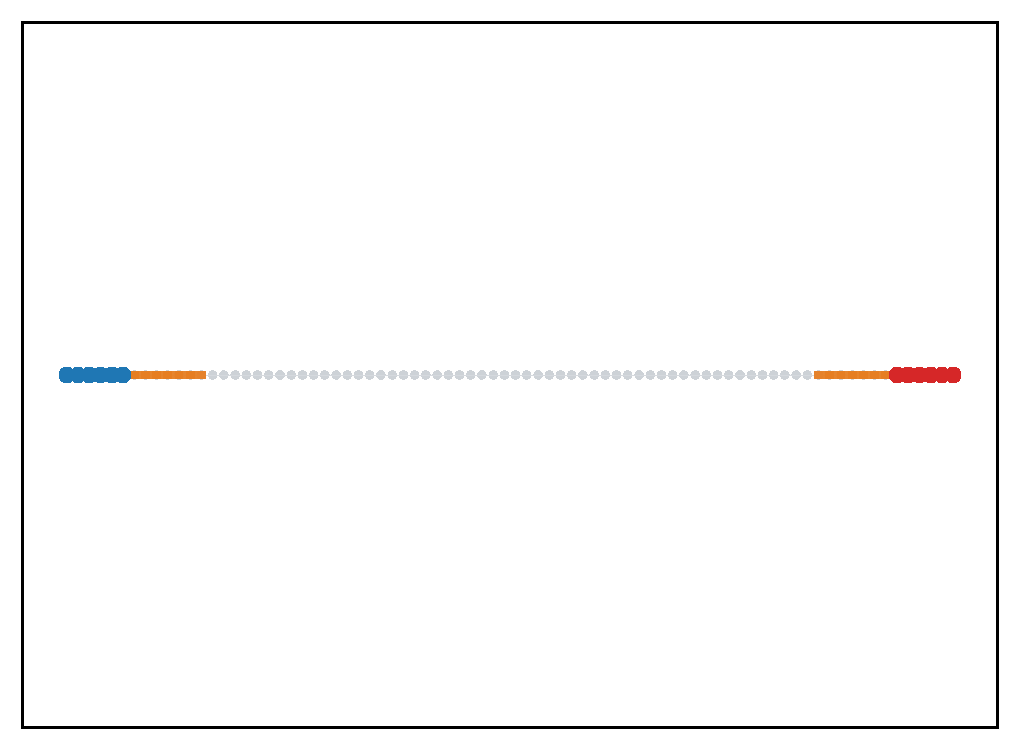
\includegraphics[width=\linewidth]{figures/benchmark-small-line-graph.pdf}
\end{minipage}\hfill
\begin{minipage}{0.3\linewidth}\centering
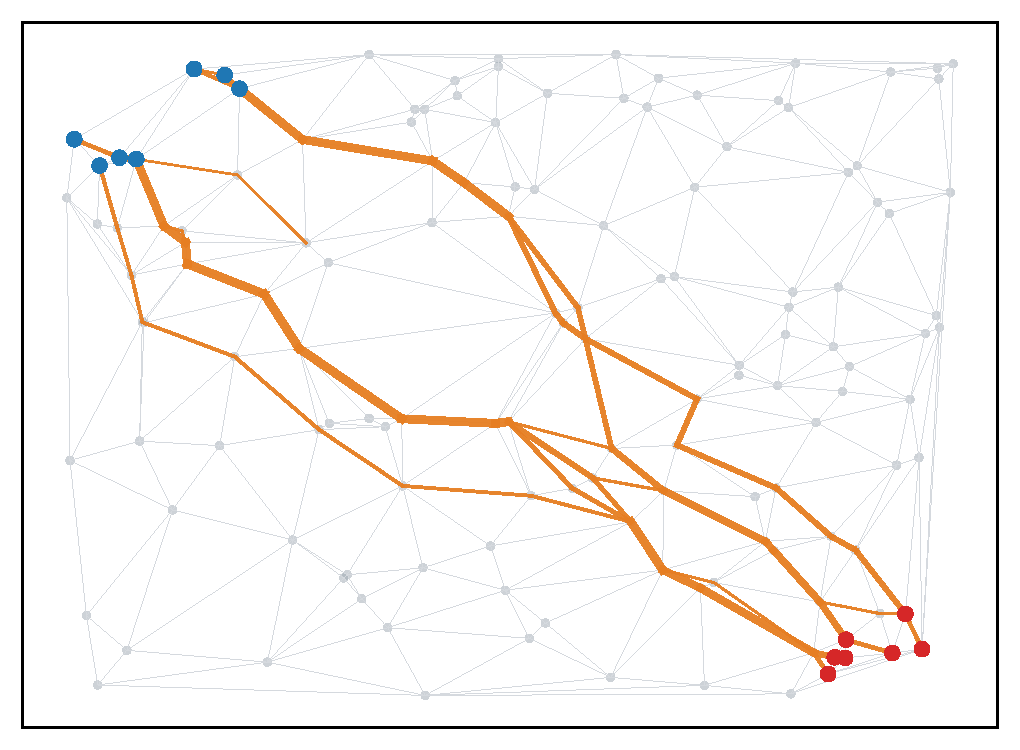
\includegraphics[width=\linewidth]{figures/benchmark-small-delaunay-graph.pdf}
\end{minipage}\hfill
\begin{minipage}{0.3\linewidth}\centering
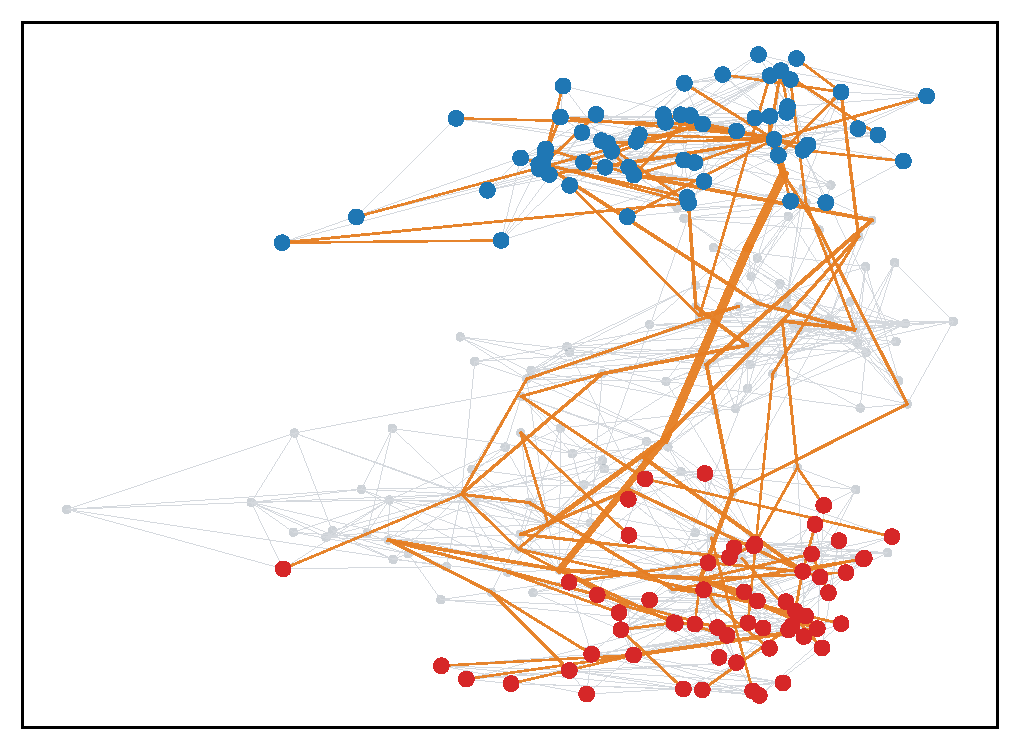
\includegraphics[width=\linewidth]{figures/benchmark-small-singlecell-graph.pdf}
\end{minipage}
% \medskip
\begin{minipage}{0.32\linewidth}\centering
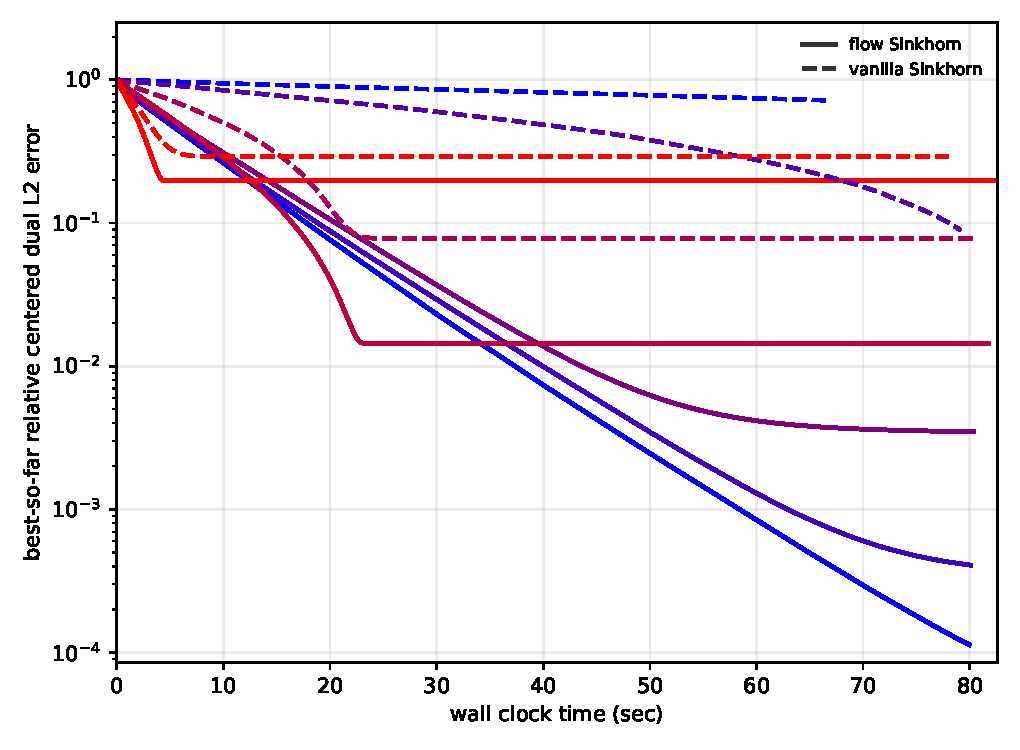
\includegraphics[width=\linewidth]{figures/benchmark-small-line-convergence.pdf}
\end{minipage}\hfill
\begin{minipage}{0.32\linewidth}\centering
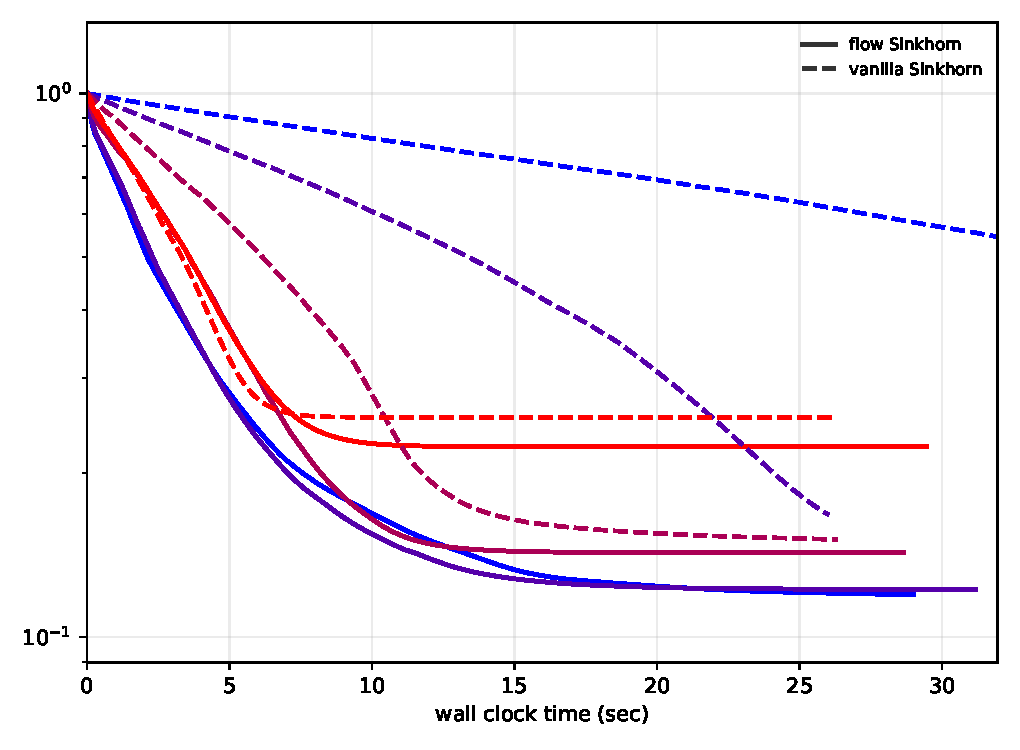
\includegraphics[width=\linewidth]{figures/benchmark-small-delaunay-convergence.pdf}
\end{minipage}\hfill
\begin{minipage}{0.32\linewidth}\centering
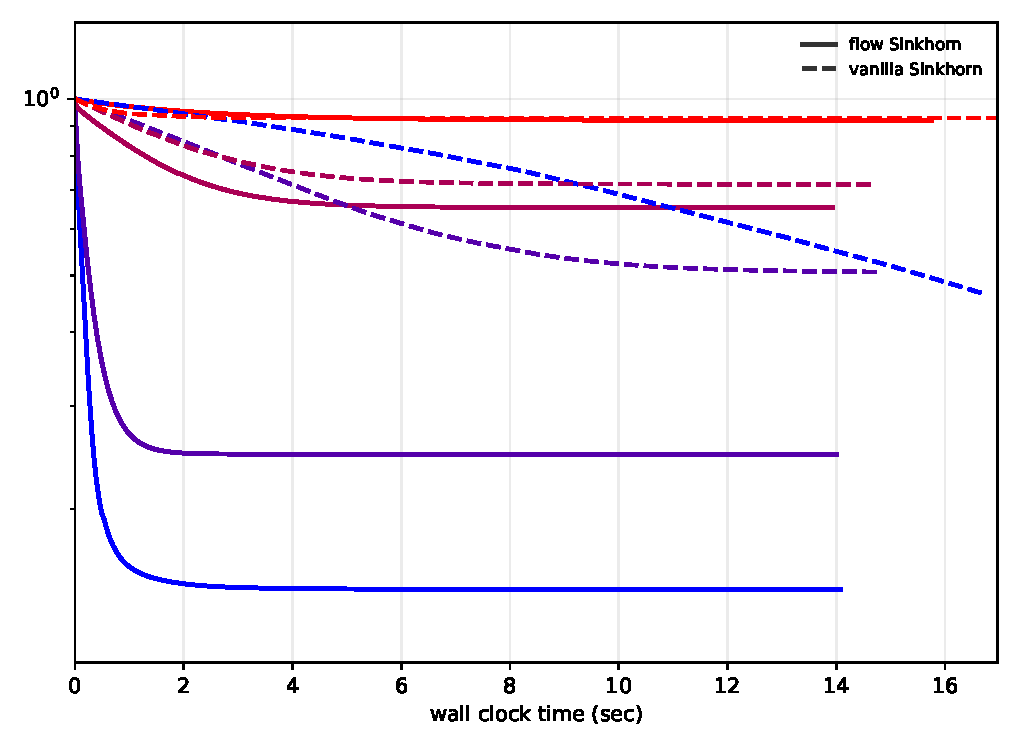
\includegraphics[width=\linewidth]{figures/benchmark-small-singlecell-convergence.pdf}
\end{minipage}\vspace{-2mm}
\caption{Top row: benched graph together with the flow $f$ (line graph, planar Delaunay, single cell). Bottom row: best-so-far relative centered dual-potential error $e(t)$, defined in the text, against wall-clock time. Flow Sinkhorn is plain and vanilla Sinkhorn is dashed; colors encode $\gamma$ from blue (small) to red (large).
Gamma ranges are: line (flow $\gamma\in[10^{-3},5]$, vanilla $\gamma\in[10^{-1},1]$), Delaunay (flow $\gamma\in[9\times10^{-4},9\times10^{-3}]$, vanilla $\gamma\in[9\times10^{-4},9\times10^{-3}]$), single-cell (flow $\gamma\in[3\times10^{-1},9]$, vanilla $\gamma\in[1,5]$).}
\label{fig:bench-overview-small}
\end{figure}

\begin{figure}[htbp]
\centering
\begin{minipage}{0.32\linewidth}\centering
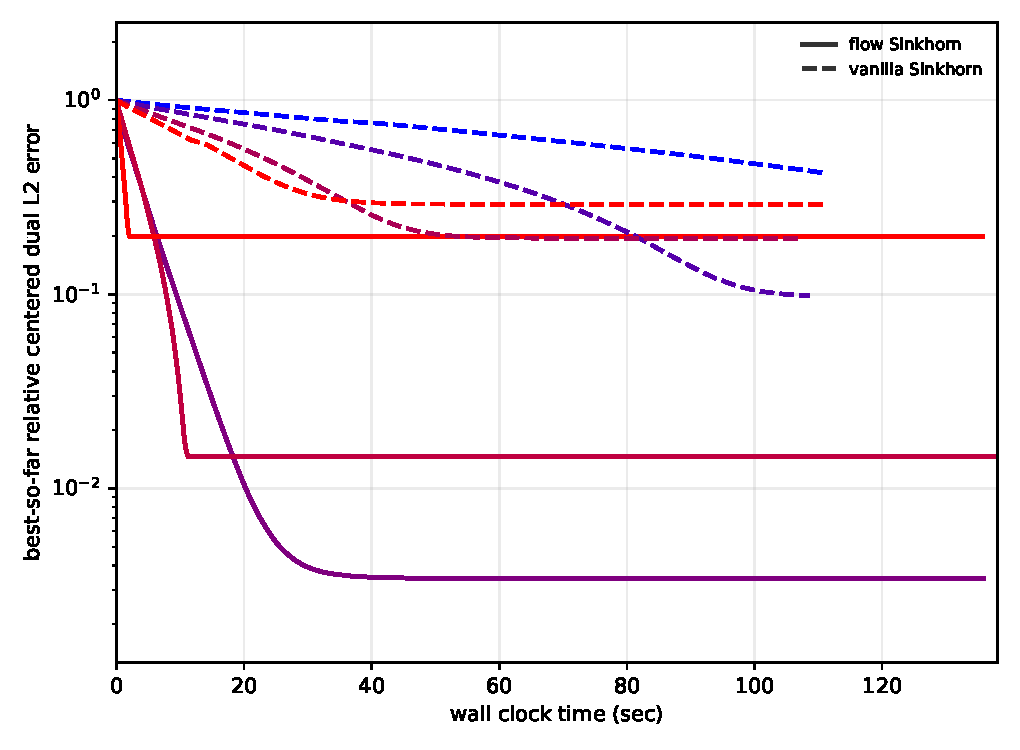
\includegraphics[width=\linewidth]{figures/benchmark-gpu-small-half-tuned-line-convergence.pdf}
\end{minipage}\hfill
\begin{minipage}{0.32\linewidth}\centering
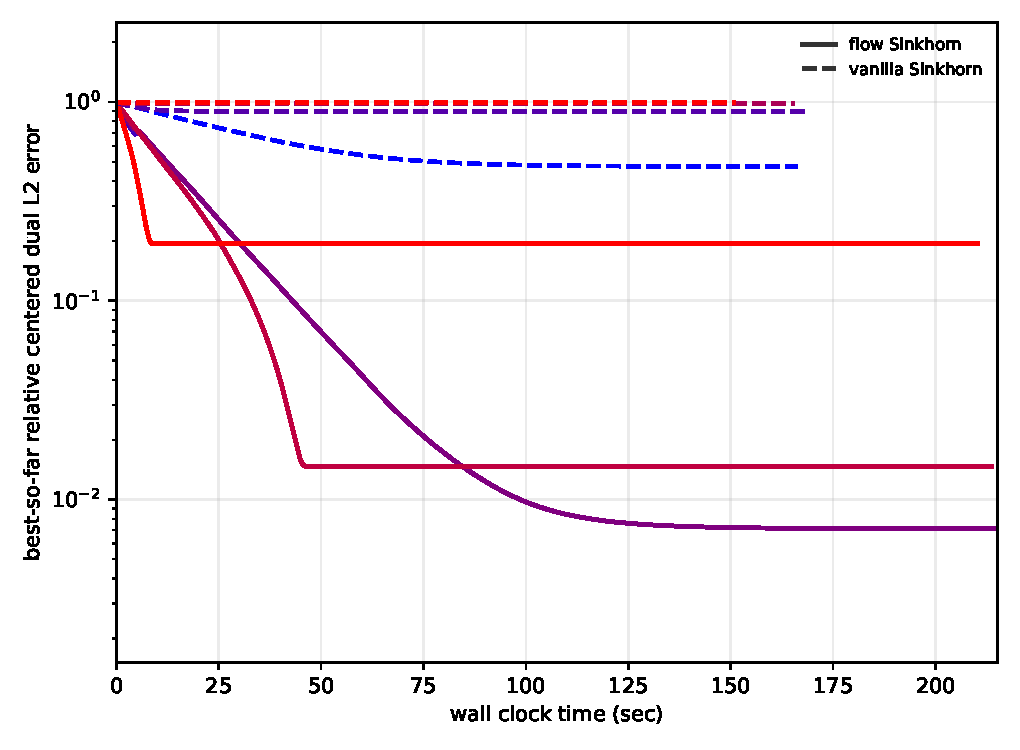
\includegraphics[width=\linewidth]{figures/benchmark-gpu-large-half-tuned-v2-line-convergence.pdf}
\end{minipage}\hfill
\begin{minipage}{0.32\linewidth}\centering
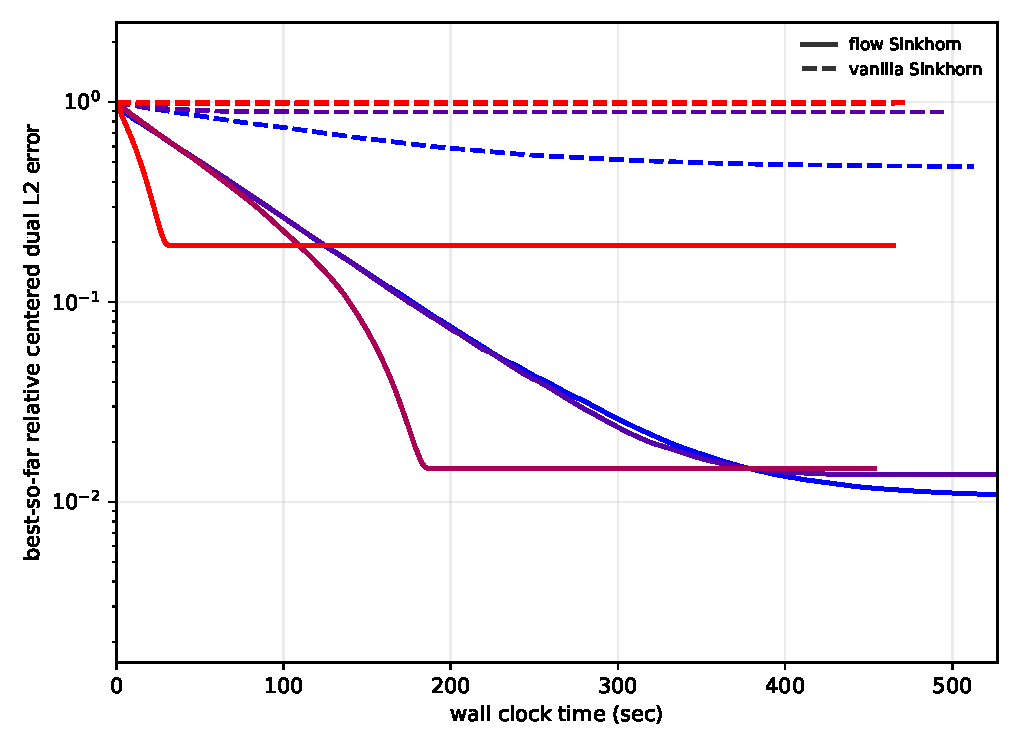
\includegraphics[width=\linewidth]{figures/benchmark-gpu-larger-half-tuned-v6-line-convergence.pdf}
\end{minipage}\vspace{-2mm}
\caption{GPU line-graph benchmark, same best-so-far relative centered dual-potential error as in Figure~\ref{fig:bench-overview-small}. From left to right: small ($n=80,m=6$), large ($n=160,m=12$), and larger ($n=320,m=24$) line-segment tests. %  Flow-Sinkhorn curves are solid and vanilla Sinkhorn curves are dashed.
}
\label{fig:bench-line-gpu-scaling}
\end{figure}


\section*{Conclusion}
A useful projection analysis must control the constants as well as the iteration count. Our blueprint isolates bounded-mass curvature, quotient geometry, and exact block ascent; the graph splitting verifies these inputs with edge-local updates. Its guarantees concern regularized dual gaps and unregularized optimal values, not a uniform rate for feasible flows or the empirical potential error. Finding stable, efficiently solvable splits for general LPs, obtaining sharper graph-dependent constants, and extending the non-expansive route to noncommutative transport remain worthwhile directions.
\section*{Acknowledgement}
This work was supported by the European Research Council (ERC project WOLF) and the French government under the management of Agence Nationale de la Recherche as part of the ``France 2030'' program, reference ANR-23-IACL-0008 (PRAIRIE-PSAI).
\paragraph{Use of language models.}
Language models assisted with mathematical consistency checks, exposition, and drafting and checking the Lean development. A compiling Lean theorem certifies its stated hypotheses and conclusion; it does not, by itself, certify that these coincide with a mathematical statement in the article. Appendix~\ref{app-sec:lean-formalization} describes this distinction and the remaining formalization work.
\bibliographystyle{plainnat}
\bibliography{references}
\clearpage
\appendix
\section{Proof of the Sublinear Dual Rate}\label{app-app:dual-rate-proofs}
\paragraph{Existence and positivity in Proposition~\ref{prop:dual-gamma-correct}.}
The function $\langle C,x\rangle+\gamma\KL(x|z)$ is continuous on $\mathbb R_+^d$, strictly convex, and coercive: each scalar entropy grows faster than linearly. Its restriction to the nonempty closed feasible set has a unique minimizer. If a coordinate of that minimizer vanished, moving a distance $t>0$ toward a strictly positive feasible point would contribute a negative $t|\log t|$ leading term in the vanishing coordinates, whereas changes at positive coordinates and in the linear cost are $O(t)$. This contradicts optimality. At an interior minimizer, the gradient annihilates $\ker A$, hence belongs to $\range A^\top$. Therefore $C+\gamma\log(x_\gamma^\star/z)=A^\top u^\star$ for some finite multiplier. Substitution into the Lagrangian gives equality of primal and dual values. The same argument applies to each individual affine block with any positive reference, proving existence and positivity of each projection and existence of a block multiplier. Strict convexity makes the primal block solution unique; a dual block multiplier is unique modulo $\ker A_s^\top$.

\begin{lemma}[Exact block ascent]\label{app-lem:per-step-ascent}
If $u^+$ is obtained from $u$ by exactly maximizing block $s$, then
$F_\gamma(u^+)-F_\gamma(u)=\gamma\KL(x(u^+)|x(u))$.
\end{lemma}
\begin{proof}
Write $x^+=x(u^+)$ and $x=x(u)$. The logarithmic ratio is $\gamma\log(x^+/x)=A_s^\top(u_s^+-u_s)$, and $A_sx^+=b_s$. Consequently
\[
\gamma\KL(x^+|x)=\langle b_s,u_s^+-u_s\rangle
-\gamma\sum_i x_i^++\gamma\sum_i x_i
=F_\gamma(u^+)-F_\gamma(u).
\]
No equal-mass assumption is used. The order of the arguments of KL is important.
\end{proof}

\begin{lemma}[Gap versus residual in the quotient]\label{app-lem:gap-vs-res-quotient}
At any $u$ with $A_2x(u)=b_2$, put $r_1=b_1-A_1x(u)$. Then $r_1\perp N_1$ and
$F_\gamma^\star-F_\gamma(u)\leq(\|u_1^\star\|_{V_1}+\|u_1\|_{V_1})\|r_1\|_1$.
\end{lemma}
\begin{proof}
For $h\in\ker A^\top$, feasibility gives $\langle h,b\rangle=0$, and $\langle h,Ax(u)\rangle=0$. Because the second residual is zero, $\langle h_1,r_1\rangle=0$ for every $h_1\in N_1$. Concavity yields $F_\gamma^\star-F_\gamma(u)\leq\langle u_1^\star-u_1,r_1\rangle$. Shift $u_1^\star$ and $u_1$ independently by elements of $N_1$, apply $\ell^1$--$\ell^\infty$ duality, and take the two infima. A common gauge is not required because the second residual vanishes.
\end{proof}

\begin{proposition}[Normalized Pinsker inequality]\label{app-prop:pinsker-normalized}
For probability vectors $p,q$, $\KL(p|q)\geq\tfrac12\|p-q\|_1^2$.
\end{proposition}
\begin{proof}
This is the case $X=1$ of the following lemma. The convention $p_i>0,q_i=0\Rightarrow\KL(p|q)=+\infty$ includes boundary distributions.
\end{proof}

\begin{lemma}[Non-normalised Pinsker inequality]\label{app-lem:pinsker-nonnormalized}
If $p,q\geq0$ and $\max(\|p\|_1,\|q\|_1)\leq X$ for $X>0$, then
\begin{equation}\label{eq:bounded-pinsker}
\KL(p|q)\geq\frac{\|p-q\|_1^2}{2X}.
\end{equation}
The masses of $p$ and $q$ may differ.
\end{lemma}
\begin{proof}
For positive vectors set $q_t=q+t(p-q)$. The integral Taylor remainder of $\sum_i x_i(\log x_i-1)$ gives
\[
\KL(p|q)=\int_0^1(1-t)\sum_i\frac{(p_i-q_i)^2}{(q_t)_i}\,dt
\geq\int_0^1(1-t)\frac{\|p-q\|_1^2}{\|q_t\|_1}\,dt
\geq\frac{\|p-q\|_1^2}{2X},
\]
where the first inequality is weighted Cauchy--Schwarz. For boundary points of finite divergence, replace $p,q$ by $p+\delta\mathbf1,q+\delta\mathbf1$, use the bound $X+d\delta$, and let $\delta\downarrow0$. Each scalar KL term converges to its extended-value limit, including $p_i=0$; if $p_i>0=q_i$, the original claim is immediate from infinite divergence. Thus the limiting argument does not rely on a reversed lower-semicontinuity inequality.
\end{proof}

\paragraph{Proof of Theorem~\ref{thm:kl-dual-rate}.}
Write $r_k=\|b_1-A_1x^{(k)}\|_1$. Lemma~\ref{app-lem:gap-vs-res-quotient} gives $\Delta_k\leq2U_\gamma r_k$. Since $A_1x^{(k+1/2)}=b_1$,
$r_k\leq a\|x^{(k+1/2)}-x^{(k)}\|_1$. Both vectors obey the mass bound, so Lemmas~\ref{app-lem:per-step-ascent} and~\ref{app-lem:pinsker-nonnormalized}, together with ascent of the second block, imply
\[
\Delta_k-\Delta_{k+1}\geq\frac{\gamma r_k^2}{2X_\gamma a^2}
\geq c\Delta_k^2,\qquad c=\frac\gamma{8X_\gamma U_\gamma^2a^2}.
\]
If a gap vanishes all later gaps vanish. Otherwise
$1/\Delta_{k+1}-1/\Delta_k=(\Delta_k-\Delta_{k+1})/(\Delta_k\Delta_{k+1})\geq c$, since $\Delta_{k+1}\leq\Delta_k$. Summation gives $\Delta_k\leq(\Delta_0^{-1}+ck)^{-1}\leq1/(ck)$. If the problem has no effective constraint ($a=0$), the Gibbs vector solves it and the gap is zero; the theorem excludes this uninteresting denominator case.

\section{Regularization Bias and Optimal-Value Accuracy}\label{app-app:kl-bias-runtime}
\begin{lemma}[KL bias]\label{app-lem:kl-bias}
For any unregularized optimizer $x_0^\star$, $0\leq F_\gamma^\star-F_0^\star\leq\gamma\KL(x_0^\star|z)$. If $\|x_0^\star\|_1\leq M$ and $z_{\min}=\min_i z_i>0$, then the positive quantity $B_0=Z+M\log\max\{1,M/z_{\min}\}$ is an admissible envelope, with the product term defined as zero for $M=0$.
\end{lemma}
\begin{proof}
KL is nonnegative, so minimizing the regularized objective cannot give a value below $F_0^\star$. Evaluating it at $x_0^\star$ proves the upper bound. For the envelope, each positive coordinate obeys $x_i\leq M$ and hence $\log(x_i/z_i)\leq\log\max\{1,M/z_{\min}\}$. Sum, use $\sum_i x_i\leq M$, and discard the nonpositive term $-\sum_i x_i$. When $M=0$, the divergence is exactly $Z$. This general bound need not be sharp, but keeps all mass and reference constants explicit.
\end{proof}
\paragraph{Proof of Theorem~\ref{thm:approx-linprog}.}
The chosen $\gamma$ makes the bias at most $\varepsilon/2$. Substitution into Theorem~\ref{thm:kl-dual-rate} gives $\Delta_K\leq16X_\gamma U_\gamma^2a^2B_0/(\varepsilon K)\leq\varepsilon/2$. Since $F_\gamma(u^{(K)})=F_0^\star+(F_\gamma^\star-F_0^\star)-\Delta_K$, the absolute error is in fact at most $\varepsilon/2$ under these conservative allocations, and in particular at most $\varepsilon$. Stating the looser $\varepsilon$ guarantee permits the usual separate bias/optimization error interpretation. A primal feasible certificate requires an additional construction and is not a consequence of this algebra alone.

\section{Extension to General Bregman Divergences}\label{app-app:general-bregman}
\paragraph{Domains and duality.}
Let $\phi$ be a Legendre convex function on a finite-dimensional primal space with norm $\|\cdot\|$, and choose $z$ in its differentiability domain. Define $D_\phi(x|z)=\phi(x)-\phi(z)-\langle\nabla\phi(z),x-z\rangle$. Consider minimizing $\langle C,x\rangle+\gamma D_\phi(x|z)$ subject to $Ax=b$. Assume strong duality with attained primal and dual optima, each exact block maximization is attained, and the points
$w(u)=\nabla\phi(z)+(A^\top u-C)/\gamma$
encountered below, including at an optimum, lie in the interior differentiability domain of $\phi^*$. These domain assumptions replace any assertion that arbitrary Bregman functions automatically admit all updates. The correct dual and recovery are
\begin{equation}\label{eq:bregman-dual}
 F_\gamma(u)=\langle b,u\rangle-\gamma\phi^*(w(u))
 +\gamma\phi^*(\nabla\phi(z)),\qquad x(u)=\nabla\phi^*(w(u)).
\end{equation}
The constant is retained for absolute-value comparisons.

\paragraph{Curvature and rate.}
Equip the constraint space with the block-sum norm $\|(r_1,r_2)\|_Y=\|r_1\|_{Y_1}+\|r_2\|_{Y_2}$ and its maximum dual norm. Form $\|\cdot\|_{V_1}$ by quotienting $\|\cdot\|_{Y_1^*}$ by $N_1$. Initialize with a second-block solve, and suppose the first-block orbit and an optimum have quotient radius $U_\gamma$. Assume
$D_\phi(x^{(k+1/2)}|x^{(k)})\geq\eta_\gamma\|x^{(k+1/2)}-x^{(k)}\|^2$
for $\eta_\gamma>0$. Set $a=\|A\|_{\|\cdot\|\to Y}>0$. Then
\begin{equation}\label{eq:bregman-rate}
 \Delta_k\leq\frac{4U_\gamma^2a^2}{\gamma\eta_\gamma k},\qquad k\geq1.
\end{equation}
Indeed, Legendre duality and the block first-order condition give the exact identity $F_\gamma(u^+)-F_\gamma(u)=\gamma D_\phi(x(u^+)|x(u))$. The quotient residual argument is unchanged, using the stated dual norms. Thus progress is at least $\gamma\eta_\gamma r_k^2/a^2$, while $\Delta_k\leq2U_\gamma r_k$, and the reciprocal recurrence proves~\eqref{eq:bregman-rate}. For KL on a bounded-mass set, $\eta_\gamma=1/(2X_\gamma)$ recovers the factor eight in Theorem~\ref{thm:kl-dual-rate}. Nonnegativity and evaluation at an unregularized optimizer similarly give $0\leq F_\gamma^\star-F_0^\star\leq\gamma D_\phi(x_0^\star|z)$. The mass helper of Proposition~\ref{prop:mass-bound-block}, however, relies on KL's exponential conjugate and is not a general Bregman identity.

\subsection{Quantum Optimal Transport as a Noncommutative Bregman Projection}\label{app-app:quantum-ot}
\paragraph{Variational problem and literature.}
Let $\rho\succ0$ and $\sigma\succ0$ be density matrices on finite-dimensional spaces of dimensions $d_1,d_2$, with trace one. For a Hermitian cost $C$ and reference $Z\succ0$ on the tensor product, consider
\begin{equation}\label{eq:qot-problem}
 \min_{P\succeq0}\ \tr(CP)+\gamma\KL(P|Z),\qquad
 \tr_2P=\rho,\quad \tr_1P=\sigma,
 \qquad
 \KL(P|Q)=\tr\big(P(\log P-\log Q)-P+Q\big).
\end{equation}
The entropy is the Umegaki relative entropy with its generalized linear terms, not an entrywise KL. With singular marginals one must first restrict to their supports. Quantum transport encompasses several distinct constructions: matrix-valued transport~\citep{ning2014matrix,peyre2019quantum}, quantum couplings~\citep{golse2016mean,caglioti2019quantum}, and learning applications~\citep{chakrabarti2019quantum}. For the partial-trace entropic formulation closest to~\eqref{eq:qot-problem}, Feliciangeli, Gerolin, and Portinale~\citep{feliciangeli2021noncommutative} already prove noncommutative Sinkhorn convergence and a priori dual estimates. Convex-regularized extensions are studied in~\citep{caputo2024quantum}. We do not claim that convergence or all forms of dual control are open in quantum information theory.

\paragraph{Dual maps.}
For Hermitian multipliers $F,G$ the dual is
\begin{equation}\label{eq:qot-dual}
 \tr(\rho F)+\tr(\sigma G)+\gamma\tr Z
 -\gamma\tr\exp\!\left(\log Z+
 \frac{F\otimes I+I\otimes G-C}{\gamma}\right).
\end{equation}
Its primal recovery is the matrix exponential appearing here. The maps $\Psi_1(G),\Psi_2(F)$ are exact variational block maximizers, characterized respectively by $\tr_2P=\rho$ and $\tr_1P=\sigma$. In the noncommuting setting these equations need not reduce to an explicit matrix log-sum-exp update; replacing their solution by an entrywise or multiplicative surrogate would change the method. The feasible set contains $\rho\otimes\sigma\succ0$ and is compact, giving a unique positive entropic optimizer. The finite-dimensional equality-constraint argument then gives a dual multiplier; the same argument proves existence of each block solution. This establishes well-posedness of the variational updates, not a closed form or uniform iteration rate.

\paragraph{Quantum Pinsker and the correct geometry.}
For trace-one positive matrices the quantum Pinsker inequality reads
\begin{equation}\label{eq:quantum-pinsker}
 \KL(P|Q)\geq\tfrac12\nucnorm{P-Q}^2,\qquad
 \nucnorm{X}=\tr\sqrt{X^*X},\qquad
 (\|\cdot\|_*)^*=\|\cdot\|_{\rm op}.
\end{equation}
One proof applies monotonicity of quantum relative entropy under the two-outcome measurement onto the positive spectral subspace of $P-Q$~\citep{hiai1981sufficiency,watrous2018theory}; the measured $\ell^1$ difference is exactly $\nucnorm{P-Q}$, and Proposition~\ref{app-prop:pinsker-normalized} applies. With equal trace $m>0$, the coefficient is $1/(2m)$ by scaling. Partial-trace projection fixes the total trace, so the coefficient $1/2$ applies at every full and half-step after the initial projection.

The adjoint kernel consists of $(cI,-cI)$. Thus each \emph{block} quotient is
$\inf_{c\in\mathbb R}\opnorm{F+cI}=\tfrac12(\lambda_{\max}(F)-\lambda_{\min}(F))$, a spectral variation seminorm. The joint quotient $\inf_c\max\{\opnorm{F+cI},\opnorm{G-cI}\}$ is a different quantity. On Hermitian matrices, each partial trace is trace-norm contractive, so the combined constraint map into the sum trace norm has operator norm at most two. Also $\kappa_1\leq1$: if $\opnorm{F\otimes I+I\otimes G}\leq L$, comparison of two eigenvalues of $F$ with a fixed eigenvalue of $G$ gives spectral variation at most $L$. These finite-dimensional geometric inputs are therefore explicit, with no hidden entrywise interpretation.

\paragraph{Remaining quantitative step.}
The Bregman theorem applies conditionally once an explicit uniform spectral-quotient radius for the exact dual orbit is established. Quantum Pinsker and the norm of the partial-trace map do not establish this radius. In particular, the matrix exponential is not operator monotone on the full Hermitian order, so the elementary scalar order proof of Proposition~\ref{app-prop:topical-nonexpansive} cannot simply be copied. This observation is not, by itself, a proof that the composite quantum block map is expansive. We do not assert non-expansiveness of that map here. Relating available quantum dual estimates~\citep{feliciangeli2021noncommutative} to explicit small-$\gamma$, marginal-spectrum, and dimension dependence sufficient for our particular complexity bound remains outside the results proved in this article. The quantum discussion consequently provides a promising additional setting and verified geometric ingredients, not a completed second complexity theorem. A cost-based trace-mass bound would require a spectral lower bound $C\succeq cI$, not entrywise positivity; here the trace constraints already fix the primal mass exactly.

\section{Proofs of the Bound Helpers}\label{app-app:primaldual-proofs}
\paragraph{Proof of Proposition~\ref{prop:uniform-iter-final}.}
The kernel of $u\mapsto A^\top u$ is contained in the kernel of $u\mapsto[u_1]\in\mathbb R^{m_1}/N_1$. Thus the latter map factors through the finite-dimensional subspace $\range A^\top$, proving finiteness of~\eqref{eq:kappa} and the inequality $\|u_1\|_{V_1}\leq\kappa_1\|A^\top u\|_\infty$. Stationarity proves the optimum bound. An optimal pair is block optimal. Any representatives selected by the exact maps differ from the corresponding optimum by block kernels, so $\Psi(u_1^\star)=u_1^\star$ in the quotient. Repeated non-expansiveness gives
$\|u_1^{(k)}-u_1^\star\|_{V_1}\leq\|u_1^{(0)}-u_1^\star\|_{V_1}$. Two applications of the triangle inequality prove the claimed orbit estimate. A representative with small ordinary infinity norm exists for each first block separately; this does not assert that both blocks can be made small by one joint gauge.

\paragraph{Proof of Proposition~\ref{prop:mass-bound-block}.}
By~\eqref{eq:dual-regul},
$\gamma\|x(u)\|_1=\langle b,u\rangle+\gamma Z-F_\gamma(u)$.
At zero, $F_\gamma(0)=\gamma Z-\gamma\sum_i z_i e^{-C_i/\gamma}$. Subtracting these expressions and using the two hypotheses proves the mass estimate. This applies to both full and half-steps, since all of them follow the preliminary block solve by ascent.

For a joint kernel shift $h$, $\langle b,h\rangle=0$ because $b\in\range A$. Therefore a simultaneous quotient radius $Q_\gamma$ bounds the pairing by $\|b\|_1Q_\gamma$. For $b_2=0$, $\langle b_1,h_1\rangle=0$ for every $h_1\in N_1$, proving the stated graph specialization. In contrast, for $A_1=A_2=[1]$ and $b_1=b_2=1$, one has $N_1=N_2=\mathbb R$, so both block seminorms vanish identically, whereas $u_1+u_2$ can be arbitrarily large. This simple example rules out deriving a general pairing bound from the maximum of the independent block seminorms.

\section{Balanced Optimal Transport Specialization}\label{app-app:sinkhorn-ot}\label{app-subsec:sinkh-analysis}
Let $a\in\mathbb R_{++}^{n_1}$ and $b\in\mathbb R_{++}^{n_2}$ be probability vectors, and let $0\leq C_{ij}\leq C_{\max}$ with $C_{\max}>0$. Zero-mass rows or columns may be removed first. Consider $P\geq0$ with $P\mathbf1=a$, $P^\top\mathbf1=b$, and reference $z=a\otimes b$. The full entropy is $\KL(P|a\otimes b)$, including its linear and reference terms as in the main text. The adjoint is $A^\top(u,v)_{ij}=u_i+v_j$, with kernel $(c\mathbf1,-c\mathbf1)$; the block seminorms are variation seminorms and $\|A\|_{1\to1}=2$.

The block maps are the negative soft transforms
\begin{equation}\label{app-eq:soft-c-transform}
 \Psi_1(v)_i=-\gamma\log\sum_j b_j e^{(v_j-C_{ij})/\gamma},\qquad
 \Psi_2(u)_j=-\gamma\log\sum_i a_i e^{(u_i-C_{ij})/\gamma}.
\end{equation}
Each is order reversing and sends a constant shift to its negative. Thus the composition is order preserving and translation equivariant, implying variation non-expansiveness by Proposition~\ref{app-prop:topical-nonexpansive}. This is a direct classical proof; a strict contraction coefficient is not needed. Every completed block enforces one probability marginal, so all full and half-step primal masses equal one after the initial block solve.

\begin{proposition}[Balanced-OT log-ratio bound]\label{app-prop:hgamma-ot}
The regularized optimum satisfies $\|\log(P_\gamma^\star/(a\otimes b))\|_\infty\leq2C_{\max}/\gamma$.
\end{proposition}
\begin{proof}
Write $P_{ij}^\star=a_i b_j s_i t_j K_{ij}$ with $K_{ij}=e^{-C_{ij}/\gamma}\in[\rho,1]$, where $\rho=e^{-C_{\max}/\gamma}$. Set $S=\sum_i a_i s_i$ and $T=\sum_j b_j t_j$. Unit total mass gives $1\leq ST\leq1/\rho$. The marginal constraints imply $s_i=1/\sum_j b_jt_jK_{ij}$ and $t_j=1/\sum_i a_is_iK_{ij}$, so their product denominator lies in $[\rho^2ST,ST]$. Consequently $\rho^2\leq s_it_jK_{ij}\leq\rho^{-2}$. Taking logarithms gives the claim. The estimate does not assume a lower bound on individual optimal entries independent of $\gamma$.
\end{proof}

\begin{proposition}[Balanced-OT quotient geometry]\label{app-prop:kappa-ot}
For this split, $\kappa_1\leq1$. In addition, every output of $\Psi_1$ has variation at most $C_{\max}/2$.
\end{proposition}
\begin{proof}
If $|u_i+v_j|\leq L$ for all $i,j$, comparing two rows using the same column gives $|u_i-u_{i'}|\leq2L$. Thus $\|u\|_{\rm Var}\leq L$. For the second assertion, the summands defining $\Psi_1(v)_i$ and $\Psi_1(v)_{i'}$ differ by factors between $e^{-C_{\max}/\gamma}$ and $e^{C_{\max}/\gamma}$. The two logarithmic sums therefore differ by at most $C_{\max}$, proving the variation bound. The same holds at an optimum.
\end{proof}

\begin{corollary}[Balanced-OT constants]\label{app-cor:ot-xgamma-ugamma}
With the main initialization, one may take $X_\gamma=1$, $U_\gamma=C_{\max}/2$, and $a=2$ in Theorem~\ref{thm:kl-dual-rate}, giving $\Delta_k\leq8C_{\max}^2/(\gamma k)$. A bias envelope is $B_0=\min\{H(a),H(b)\}$ if this is positive, where $H(a)=-\sum_i a_i\log a_i$; any positive enlargement may otherwise be used.
\end{corollary}
\begin{proof}
The mass and variation statements just proved cover all required iterates and the optimum, including the zero first block. For a feasible coupling the linear KL terms cancel, leaving $\KL(P|a\otimes b)=H(a)+H(b)-H(P)$. Conditional entropy of a finite discrete distribution is nonnegative, so $H(P)\geq\max\{H(a),H(b)\}$. This proves the bias envelope, and direct substitution proves the rate. Degenerate zero-cost or single-point problems may be solved directly instead of using positive denominators.
\end{proof}
Unlike the graph-flow specialization, this application has a $\gamma$-independent mass bound. One dense sweep costs $O(n_1n_2)$ operations. The value guarantee and feasible-coupling rounding guarantees in the transport literature are related but distinct statements.

\section{Proofs for Graph Flow-Sinkhorn}\label{app-app:w1-proofs}
This appendix proves the graph-specific inputs used in Section~\ref{sec:applications}, retaining its orientation, half-cost normalization, and reference $z$. It does not introduce a different flow problem.

\paragraph{Operators and gauges.}
The lifted constraints in~\eqref{eq-W1-flow-lifted} are $A_1(f,g)=-f\mathbf1+g^\top\mathbf1$ and $A_2(f,g)=f-g$, with right-hand side $(q,0)$. Their combined adjoint is
\begin{equation}\label{app-app-eq:At_action}
 A^\top(v,U)=(y^f,y^g),\qquad
 y^f_{ij}=-v_i+U_{ij},\qquad y^g_{ij}=v_j-U_{ij}.
\end{equation}
Each column of the stacked matrix has two entries of magnitude one, hence $\|A\|_{1\to1}=2$ (whereas $\|A_1\|_{1\to1}=1$). Connectedness implies $\ker A^\top=\{(c\mathbf1_V,c\mathbf1_E):c\in\mathbb R\}$. Thus both block quotient seminorms are variation seminorms, on different spaces, and the paired translation parameter in Proposition~\ref{app-prop:translation-equivariance} is $\tau=+1$. The independent block quotients still need not admit simultaneous centering.

\paragraph{Proof of Proposition~\ref{prop:graphw1-projection-closed-form}.}
For a $\mathcal C_1$ multiplier $\lambda_i$, stationarity of the KL projection gives $f'_{ij}=e^{\lambda_i}f_{ij}$ and $g'_{ij}=e^{-\lambda_j}g_{ij}$. Write $s_i=e^{\lambda_i}>0$. The constraint is $-r_is_i+c_i/s_i=q_i$, whose unique positive solution is the displayed quadratic root. On $\mathcal C_2$ the scalar objective $\KL(h_{ij}|f'_{ij})+\KL(h_{ij}|g'_{ij})$ has derivative $\log(h_{ij}/f'_{ij})+\log(h_{ij}/g'_{ij})$; its zero is $\sqrt{f'_{ij}g'_{ij}}$. This proves the projection and the full sweep~\eqref{eq:proj-sinkh-flow}.

\paragraph{Proof of Proposition~\ref{prop:graphw1-flow-sinkhorn-update}.}
Multiplication by $\sqrt{s_i/s_j}$ sends $v$ to $v-\frac\gamma2\log s$. For a full iterate, $r_i=e^{-v_i/\gamma}e^{\alpha_i^+/\gamma}$ and $c_i=e^{v_i/\gamma}e^{\alpha_i^-/\gamma}$. The quadratic root satisfies
$\log s_i=\tfrac12(\log c_i-\log r_i)-\arsinh(q_i/(2\sqrt{r_ic_i}))$.
Substituting in the potential update gives~\eqref{eq:v-update-stable}. To evaluate its last term, set $\ell_i=\log(|q_i|/2)-(\alpha_i^++\alpha_i^-)/(2\gamma)$ when $q_i\ne0$. For $\ell\geq0$, use $\arsinh(e^\ell)=\ell+\log(1+\sqrt{1+e^{-2\ell}})$; for $\ell<0$, $\arsinh(e^\ell)$ has a bounded argument. Multiply by $\sign q_i$, and return zero if $q_i=0$. This avoids forming a possibly overflowing exponential of $\ell_i>0$.

\begin{proposition}[Graph block maps and non-expansiveness]\label{prop:graphw1-psi2-closed-nonexp}
With the normalized adjoint~\eqref{app-app-eq:At_action}, $\Psi_2(v)_{ij}=(v_i+v_j)/2$. The first block $\Psi_1(U)_i$ is the unique root $t$ of
\begin{equation}\label{eq:graph-moment}
 \sum_j z_{ji}e^{(t-U_{ji}-W_{ji}/2)/\theta}
 -\sum_j z_{ij}e^{(-t+U_{ij}-W_{ij}/2)/\theta}=q_i,
 \qquad\theta=\gamma/2.
\end{equation}
Both blocks are order preserving and commute with constant translations. Consequently their composition is non-expansive in $\|\cdot\|_{\rm Var}$.
\end{proposition}
\begin{proof}
Second-block optimality says $f_{ij}=g_{ij}$. Their common reference and cost cancel in the log ratio, giving $-v_i+U_{ij}=v_j-U_{ij}$ and the average formula. Substituting it gives the physical recovery $f_{ij}=z_{ij}e^{(v_j-v_i-W_{ij})/\gamma}$. First-block optimality is exactly~\eqref{eq:graph-moment}. Its left-hand side is continuous, strictly increasing in $t$, and tends to $-\infty,+\infty$ at the two ends; every vertex has an incident edge. Each incident $U$ coordinate enters with a negative derivative, including those in the subtracted sum. Proposition~\ref{app-prop:block-monotone} therefore makes its root order preserving. Adding $c$ to all edge coordinates and to $t$ leaves the equation unchanged. The average formula has the same translation law and is order preserving. Apply Proposition~\ref{app-prop:topical-nonexpansive} to the composition. This direct scalar proof avoids assuming an order-preserving inverse for an arbitrary coupled moment map.
\end{proof}

\begin{lemma}[Positive costs bound optimal primal mass]\label{app-lem:l1-bound-from-feasible}
For a feasible problem with coordinate costs at least $c_{\min}>0$, a positive reference, and any feasible comparison $\bar x\geq0$, its regularized optimizer satisfies
$\|x_\gamma^\star\|_1\leq(\langle C,\bar x\rangle+\gamma\KL(\bar x|z))/c_{\min}$.
\end{lemma}
\begin{proof}
Nonnegativity of KL and of $x_\gamma^\star$ gives
$c_{\min}\|x_\gamma^\star\|_1\leq\langle C,x_\gamma^\star\rangle\leq F_\gamma^\star\leq\langle C,\bar x\rangle+\gamma\KL(\bar x|z)$.
\end{proof}
This elementary lemma is of independent interest beyond graph transport; its coordinatewise lower-cost hypothesis is specific to the positive-orthant/$\ell^1$ geometry.

\begin{proposition}[Graph log-ratio bound]\label{app-prop:hgamma-graphw1}
For the physical regularized optimum, $\|\log(f_\gamma^\star/z)\|_\infty\leq H_\gamma$, with $M_\gamma,H_\gamma$ from~\eqref{eq:graph-constants}. The same bound applies to the duplicated lifted optimum.
\end{proposition}
\begin{proof}
The preceding lemma bounds each coordinate of $f_\gamma^\star$ by $M_\gamma$. If $r_{ij}=\log(f_{ij}^\star/z_{ij})$, then $r_{ij}\leq\log M_\gamma+L_z$. The recovery formula in Proposition~\ref{prop:graphw1-psi2-closed-nonexp} gives
$r_{ij}+r_{ji}=-2W_{ij}/\gamma$.
Applying the upper bound to $r_{ji}$ yields $r_{ij}\geq-2W_{\max}/\gamma-\log M_\gamma-L_z$. Replacing $\log M_\gamma$ by $|\log M_\gamma|$ gives the claimed safe two-sided bound. Positivity of $M_\gamma$ follows because a zero numerator would require simultaneously zero transport cost and zero KL, impossible for $W>0,z>0$.
\end{proof}

\begin{proposition}[Graph geometry and orbit bounds]\label{app-prop:kappa-graph-diameter}
For the normalized lift, $\kappa_1\leq\Dhop$. The zero-start vertex potentials, their first-block half-steps, and an optimal vertex potential have variation radius at most $U_\gamma$ in~\eqref{eq:graph-constants}. Every full and half-step lifted primal vector has mass at most $X_\gamma$ there.
\end{proposition}
\begin{proof}
If $\|A^\top(v,U)\|_\infty\leq1$, then $v_j-v_i=y^f_{ij}+y^g_{ij}$ has magnitude at most two on each edge. A minimum-hop path gives $\max v-\min v\leq2\Dhop$, hence $\|v\|_{\rm Var}\leq\Dhop$. Applying Proposition~\ref{prop:uniform-iter-final} with $\theta=\gamma/2$ and $\|\bar C\|_\infty=W_{\max}/2$ proves the stated $U_\gamma$. Half-step first blocks equal the next full first blocks. Since $\sum_iq_i=0$, the pairing obeys $\langle q,v\rangle\leq\|q\|_1\|v\|_{\rm Var}$. Proposition~\ref{prop:mass-bound-block} with the lifted reference sum $2Z$ and cost lower bound $W_{\min}/2$ proves $X_\gamma$. In particular the coefficient $2/\gamma$ comes from the lifted regularization, not from a new normalization of $q$.
\end{proof}

\paragraph{Constructing the comparison and the bias envelope.}
A feasible $\bar f$ can be constructed on any spanning tree: for each edge, remove it, sum $q$ on either component, and send that signed excess toward the other component using the corresponding orientation. At each vertex the net outgoing flow is $q_i$. Equivalently, couple positive and negative parts of $q$ and route that coupling along tree paths. Its total path mass is at most $(n-1)\|q\|_1/2$. This constructs the finite comparison constants without solving the transport problem; the maximum tree path length should not be identified with $\Dhop$. Alternatively, route along minimum-hop graph paths if a hop-diameter comparison is desired.

For the bias envelope one needs an \emph{optimal} flow, not merely this tree comparison. Couple $q_+$ to $q_-$, whose common mass is $\|q\|_1/2$, using the weighted geodesic cost and an optimal coupling. Such a coupling exists in a finite-dimensional transport polytope. Route it along weighted shortest paths, chosen simple because all edge costs are positive. The resulting optimal flow has mass at most $M_0=(n-1)\|q\|_1/2$. The equivalence with~\eqref{eq-W1-flow} follows by discarding cycles in any feasible flow and using shortest-path lower bounds for each remaining path. Lemma~\ref{app-lem:kl-bias} now supplies the stated $B_0$, without requiring this optimizer to be computed by the algorithm.

\paragraph{Proof of Theorem~\ref{thm:graphw1-complexity}.}
The preceding propositions verify Theorem~\ref{thm:kl-dual-rate} on the normalized lift with $a=2$, parameter $\theta=\gamma/2$, and lifted mass $X_\gamma$. Thus the physical gap obeys $\Delta_k\leq64X_\gamma U_\gamma^2/(\gamma k)$. The physical bias is at most $\gamma B_0$; equivalently, the lifted bias is bounded by $\theta(2B_0)$. With $\gamma=\varepsilon/(2B_0)$, making the gap at most $\varepsilon/2$ requires $K\geq256B_0X_\gamma U_\gamma^2/\varepsilon^2$. Evaluation of the sparse dual and a full sweep both take $O(p)$ operations. Graph construction, the chosen comparison flow, and any optional reference solver are preprocessing and are not counted as sweeps. Arithmetic counts do not include a bit-complexity or finite-precision analysis.

For fixed data, $\gamma H_\gamma=2W_{\max}+\gamma L_z+\gamma|\log M_\gamma|$ remains bounded as $\gamma\downarrow0$: $M_\gamma$ is a positive affine function of $\gamma$, possibly proportional to $\gamma$ when the comparison flow is zero. Hence $U_\gamma=O(1)$ and $X_\gamma=O(1/\gamma)$. Substitution gives $K=O(\varepsilon^{-3})$. No exponential term has been dropped in the nonasymptotic bound, and no impossible condition such as $p=o(1/\log(1/\varepsilon))$ is needed. Dependence on graph size, costs, reference, and geometry is entirely retained in~\eqref{eq:graph-constants} and $B_0$.

\paragraph{Residual correction.}
For a nonnegative iterate $f$, let $r=q-Bf$. Since $\sum_i r_i=0$, pair its positive and negative parts, of mass $\|r\|_1/2$, and route along shortest paths to obtain $g\geq0$ with $Bg=r$ and $\langle W,g\rangle\leq\Dweight\|r\|_1/2$. Then $f+g$ is feasible. This proves the correction statement in the main text, not an additional iteration bound for achieving a prescribed residual. A complementary unregularized dual lower bound is obtained from a potential $v$ by dividing it by $\max\{1,\max_E|v_j-v_i|/W_{ij}\}$; the resulting potential satisfies all graph Lipschitz constraints. Such a feasible primal/dual pair gives a computable stopping certificate distinct from the regularized-dual value estimator.

\section{Non-expansiveness in the Variation Seminorm}\label{app-sec:non-expansiveness}
For $v\in\mathbb R^m$, define
\begin{equation}\label{app-eq:variation-seminorm}
\|v\|_{\rm Var}:=\inf_{c\in\mathbb R}\|v+c\mathbf1\|_\infty
=\tfrac12(\max_i v_i-\min_i v_i).
\end{equation}
The minimum is achieved by centering the largest and smallest coordinates. This is the quotient by constants, not generally the block quotient for an arbitrary split.

\begin{proposition}[Order and translations imply non-expansiveness]\label{app-prop:topical-nonexpansive}
If $T:\mathbb R^m\to\mathbb R^\ell$ is order preserving and $T(v+c\mathbf1)=T(v)+c\mathbf1$ for every real $c$, then $\|T(v)-T(w)\|_{\rm Var}\leq\|v-w\|_{\rm Var}$.
\end{proposition}
\begin{proof}
Let $a=\min_i(v_i-w_i)$ and $b=\max_i(v_i-w_i)$. Applying the two hypotheses to $w+a\mathbf1\leq v\leq w+b\mathbf1$ gives $T(w)+a\mathbf1\leq T(v)\leq T(w)+b\mathbf1$. The output oscillation is at most $b-a$. Division by two proves the result. This elementary argument is related to the general order/non-expansiveness principle in~\citep{candrall1980some}.
\end{proof}

\begin{proposition}[Scalar inverse criterion for block monotonicity]\label{app-prop:block-monotone}
Suppose each coordinate of a block optimizer is the unique scalar solution $t=T_i(w)$ of $M_i(t,w)=b_i$, where $M_i$ is strictly increasing in $t$ and continuous, with limits $-\infty,+\infty$ as $t\to-\infty,+\infty$. If $M_i(t,w)$ is order reversing in $w$, then $T_i$ is order preserving in $w$; if it is order preserving in $w$, then $T_i$ is order reversing. Consequently the composition of two order-preserving blocks, or of two order-reversing blocks, is order preserving.
\end{proposition}
\begin{proof}
In the order-reversing case, $w\leq w'$ gives $M_i(T_i(w),w')\leq b_i=M_i(T_i(w'),w')$. Strict increase in the scalar variable implies $T_i(w)\leq T_i(w')$. Reversing the inequality gives the other case. Composing two inequalities proves the final assertion. The separable scalar hypothesis is essential: positive coefficients in a coupled vector moment map do not, by themselves, make its inverse order preserving.
\end{proof}

\begin{proposition}[Translation equivariance from a paired kernel]\label{app-prop:translation-equivariance}
Assume $A_1^\top\mathbf1+\tau A_2^\top\mathbf1=0$ with $\tau\in\{-1,1\}$, and that exact block optimizers are unique (or represented consistently modulo their block kernels). Then
$\Psi_2(v+c\mathbf1)=\Psi_2(v)+\tau c\mathbf1$ and
$\Psi_1(w+\tau c\mathbf1)=\Psi_1(w)+c\mathbf1$,
with quotient equalities when necessary. In particular the full first-block sweep commutes with constant translations.
\end{proposition}
\begin{proof}
Feasibility gives $\langle b_1,\mathbf1\rangle+\tau\langle b_2,\mathbf1\rangle=0$. The paired shift $(c\mathbf1,\tau c\mathbf1)$ is in $\ker A^\top$, so it preserves the full dual objective. Changing variables by the matching shift in each block optimization identifies its argmax set with the translate of the original argmax set. Uniqueness, or the stated quotient convention, yields the formulas. No choice of arbitrary representatives is silently assumed equivariant.
\end{proof}

\section{Lean Development and Certification Scope}\label{app-sec:lean-formalization}
The repository contains a substantial Lean development of finite-dimensional inequalities, quotient geometry, scalar convergence recurrences, and conditional convergence interfaces. Organizing these reusable results independently of the article is useful: KL inequalities and recurrence lemmas, for example, have applications beyond transport. The entry point is \texttt{FlowSinkhorn.KLProjection}; thematic modules group analysis, bounds, geometry, applications, and certification infrastructure. \texttt{StatementMap.lean} provides stable aliases to historical paper-facing endpoints rather than new proofs.

\paragraph{What a successful build certifies.}
Lean checks a theorem under its declared assumptions. A theorem that assumes a bias estimate, a mass bound, an objective-gap inequality, or an already constructed certificate does not prove those ingredients. An alias to such a theorem, a generated comparison interface, and an absence of \texttt{sorry} do not establish that the article's original variational assumptions imply its conclusion. In particular, compiling the current project is not an end-to-end certificate for every statement of this revised article. The revised bounded-mass lemma, initialization, normalized graph constants, quotient pairing distinction, and graph scalar-order argument require statement-level synchronization and, in some cases, additional formal proofs.

\paragraph{Current status and reproduction.}
The revision audit is recorded in \texttt{lean/PAPER\_COVERAGE.md}. Historical statement aliases are retained to avoid breaking downstream imports, but their numerical labels must not be read as the revised paper's numbering. Running \texttt{lake build} in \texttt{lean/} checks the available Lean sources against the pinned toolchain and dependencies. It does not check this PDF, scientific relevance of assumptions, or external numerical experiments. The CI build has the same scope. The project is therefore best described as a partially formalized companion library with conditional interfaces; completion requires independent comparison of each Lean statement's hypotheses and conclusion with its mathematical counterpart, followed by formalization of every missing bridge. No percentage or blanket ``fully formalized'' claim is made here.

\section{Notation}\label{app:notation}
\begingroup
\renewcommand{\arraystretch}{1.1}
\begin{longtable}{@{}p{.27\textwidth}p{.68\textwidth}@{}}
\toprule\textbf{Notation}&\textbf{Meaning}\\\midrule\endfirsthead
\toprule\textbf{Notation}&\textbf{Meaning}\\\midrule\endhead
$d$, $A=(A_1;A_2)$ & Primal dimension and stacked affine constraint operator.\\
$b=(b_1;b_2)$, $C$ & Generic right-hand side and linear cost.\\
$z>0$, $Z=\sum_i z_i$ & Generic positive KL reference and its total mass.\\
$\gamma$, $\varepsilon$ & Physical regularization strength and target optimal-value accuracy.\\
$\mathcal C_s$ & Closed nonnegative affine constraint block $A_sx=b_s$.\\
$\KL(x|z)$ & Generalized KL, $\sum_i[x_i\log(x_i/z_i)-x_i+z_i]$.\\
$z^C$ & Gibbs reference $z\exp(-C/\gamma)$.\\
$F_0^\star$, $F_\gamma^\star$ & Unregularized and regularized primal optimal values.\\
$F_\gamma(u)$, $x(u)$ & Dual objective (including its constant) and primal recovery.\\
$u^{(k+1/2)}$, $u^{(k+1)}$ & First-block half-step and subsequent full iterate.\\
$\Psi_s$, $\Psi$ & Exact block maximizers and first-block sweep $\Psi_1\circ\Psi_2$.\\
$N_s$, $\|\cdot\|_{V_s}$ & Projection of $\ker A^\top$ onto block $s$, and quotient infinity seminorm.\\
$\|u\|_V$, $Q_\gamma$ & Maximum of independent block seminorms; separately, a simultaneous quotient-radius bound.\\
$\Delta_k$ & Regularized dual gap $F_\gamma^\star-F_\gamma(u^{(k)})$.\\
$a=\|A\|_{1\to1}$ & Constraint operator norm in the KL analysis.\\
$X_\gamma$ & Mass bound for both full and half-step primal iterates.\\
$U_\gamma$ & First-block quotient-radius bound for the orbit and an optimum.\\
$P_\gamma$ & Upper bound for the dual pairing $\langle b,u\rangle$.\\
$H_\gamma$, $\kappa_1$ & Optimum log-ratio bound and adjoint-to-first-block quotient constant.\\
$B_0$ & Positive upper bound for the regularization divergence of an unregularized optimizer.\\
$V,E,n,p$ & Graph vertices, directed edge entries, and their respective counts.\\
$W_{ij}$, $W_{\min},W_{\max}$ & Positive symmetric graph-edge costs and their bounds.\\
$D_{ij}$, $\Dweight$, $\Dhop$ & Weighted geodesic distance, weighted diameter, and unweighted hop diameter.\\
$q=b_1-b_2$ & Graph source-minus-target vector; distinct from the positive entropy reference $z$.\\
$f_{ij}$, $Bf$ & Flow from $j$ to $i$; outgoing-minus-incoming divergence.\\
$(f,g)$, $\bar C$, $\theta$ & Lifted flows, half-cost $(W/2,W/2)$, and lifted parameter $\gamma/2$.\\
$K=z e^{-W/\gamma}$ & Positive edge Gibbs kernel.\\
$v,U$ & Graph vertex and edge dual variables; $U$ is not the bound $U_\gamma$.\\
$\|v\|_{\rm Var}$ & Half oscillation $(\max v-\min v)/2$.\\
$\bar f$, $M_\gamma$, $M_0$ & Feasible comparison flow, regularized optimum mass bound, and unregularized optimal mass envelope.\\
$m$ (experiments) & Number of vertices supporting each endpoint measure, not the number of edges.\\
$e(t)$, $\widetilde v$ & Best-so-far relative dual-potential diagnostic and mean-centered potential.\\
$D_\phi$, $\eta_\gamma$ & General Bregman divergence and quadratic lower-bound constant.\\
$\rho,\sigma,P,Z$ & Quantum marginals, coupling, and positive matrix reference (uppercase $Z$ is local to the quantum subsection).\\
$\tr_1,\tr_2$ & Partial traces on the tensor-product matrix space.\\
$\|\cdot\|_*,\|\cdot\|_{\rm op}$ & Nuclear (trace) norm and its dual operator norm.\\
$F,G$ (quantum) & Hermitian dual multipliers, with gauge $(cI,-cI)$.\\
\bottomrule
\end{longtable}
\endgroup

\end{document}
